% \begin{figure}[p]
% \vspace*{2mm}
% \begin{center}
% 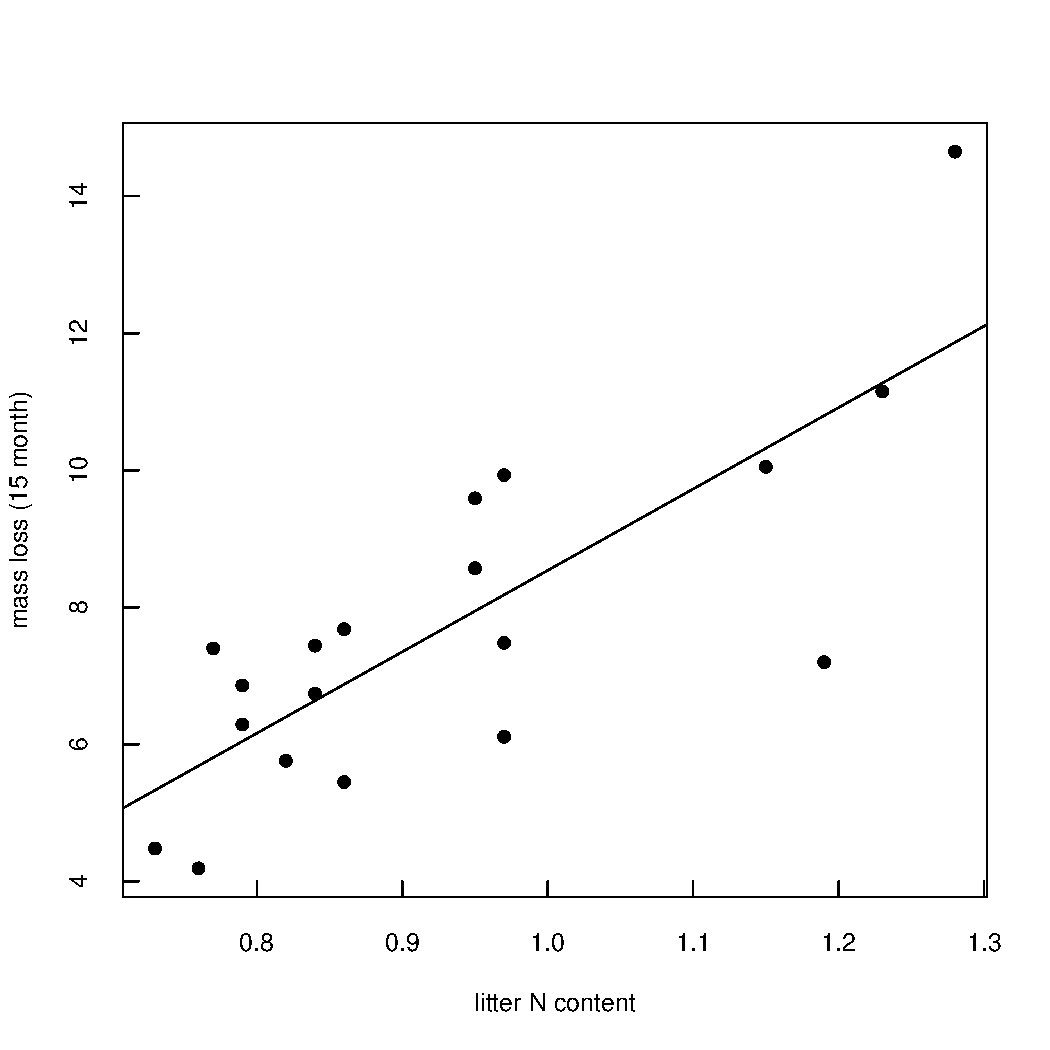
\includegraphics[width=8.3cm]{massloss_n_lit.pdf}
% \end{center}
% \label{fig:n_massloss}
% \caption{Litter mass loss after 15 month vs. litter N content. R= 0.795, p \textless .001}
% \end{figure}

% \newpage
% \begin{figure}[p]
% \vspace*{2mm}
% \begin{center}
% 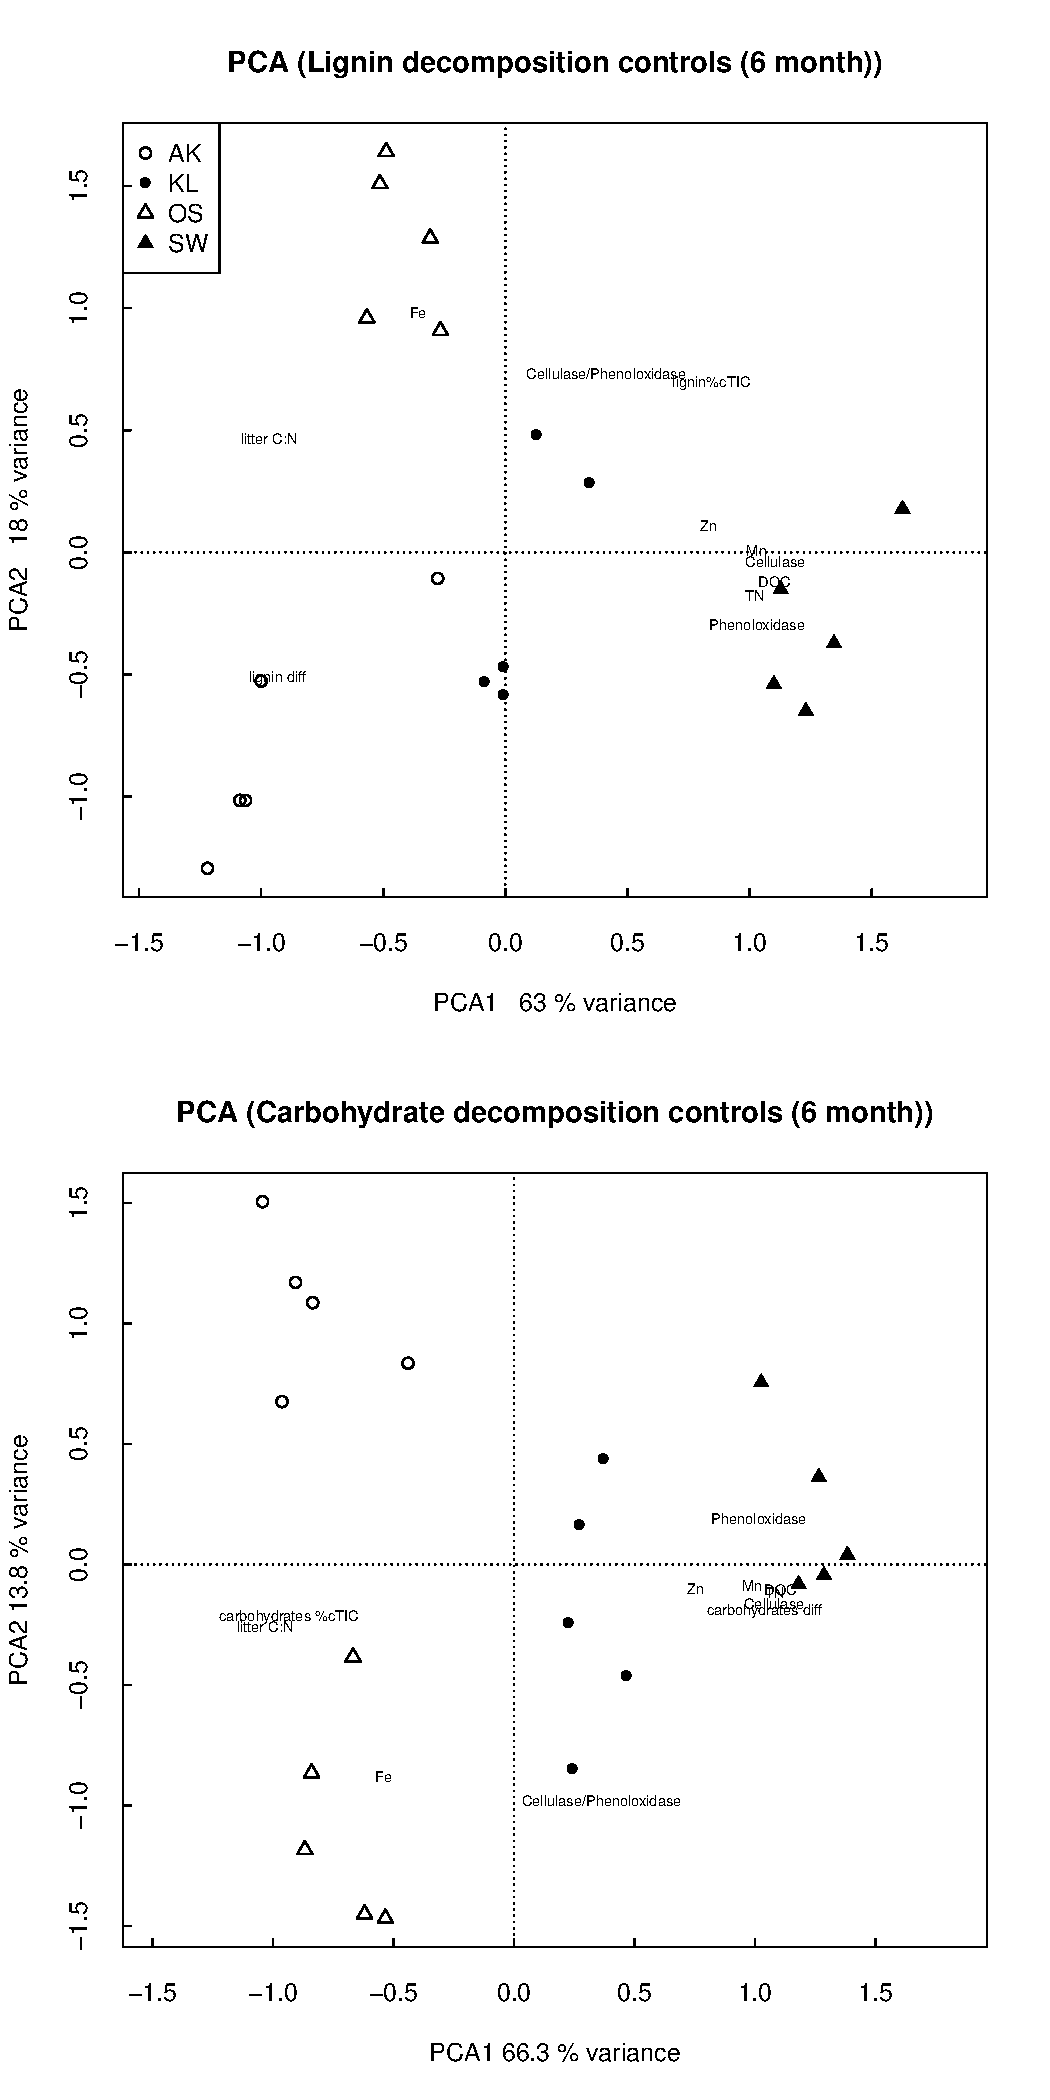
\includegraphics[width=8.3cm]{h3_decomp_contr.pdf}
% \end{center}
% \caption{Litter mass loss after 15 month vs. litter N content. R= 0.795, p \textless .001}
% \label{fig:h3_controls}
% \end{figure}

% \newpage
% \begin{figure*}[p]
% \vspace*{2mm}
% \begin{center}
% 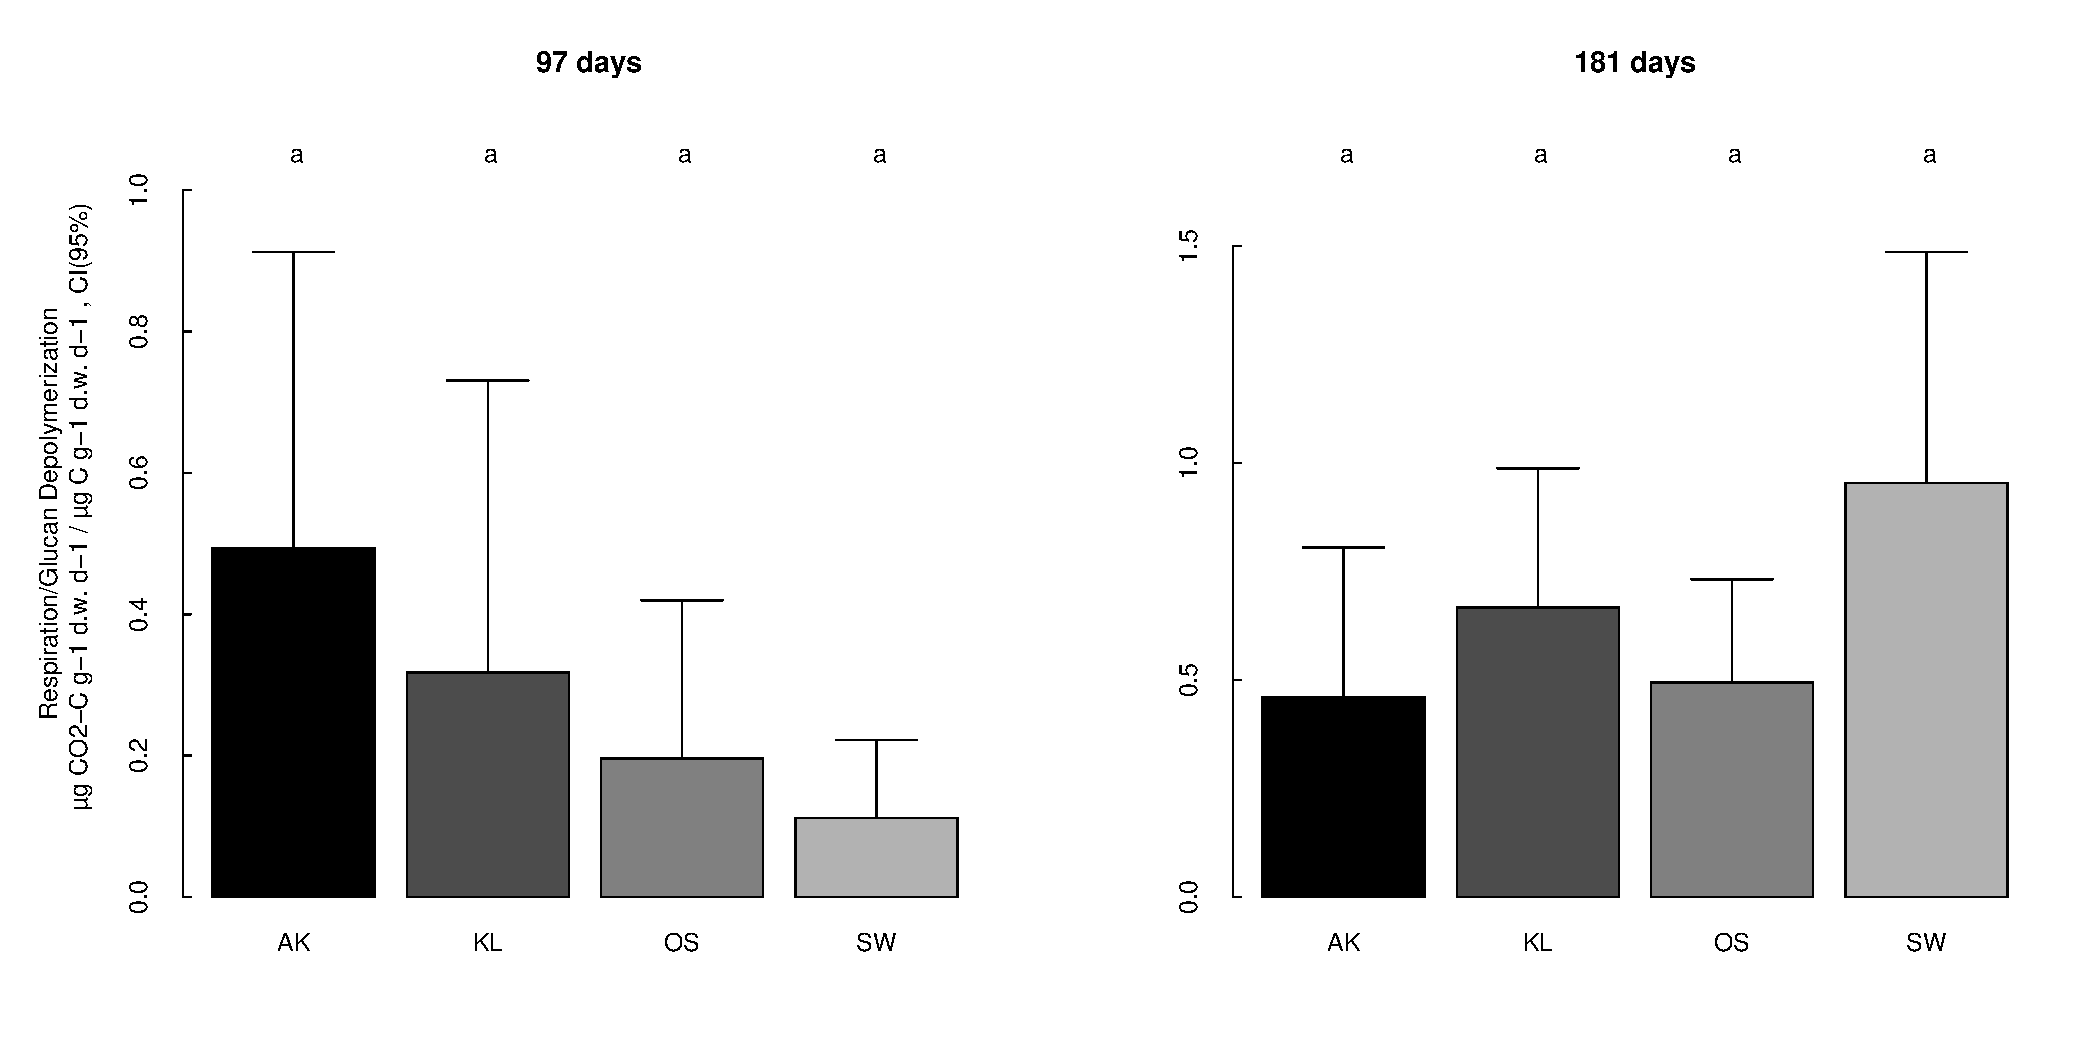
\includegraphics[width=12cm]{resp_glcdepoly_h23.pdf}
% \end{center}
% \caption{Quotient of respiration and glucan depolymerization. In AK microbial community respire significantly more non-glucose carbon after 2, but not after 6 month. Data from \cite{Leitner2011}}
% \label{fig:resp_depoly}
% \end{figure*}

\newpage
\begin{figure*}[p]
\vspace*{2mm}
% \begin{center}
% 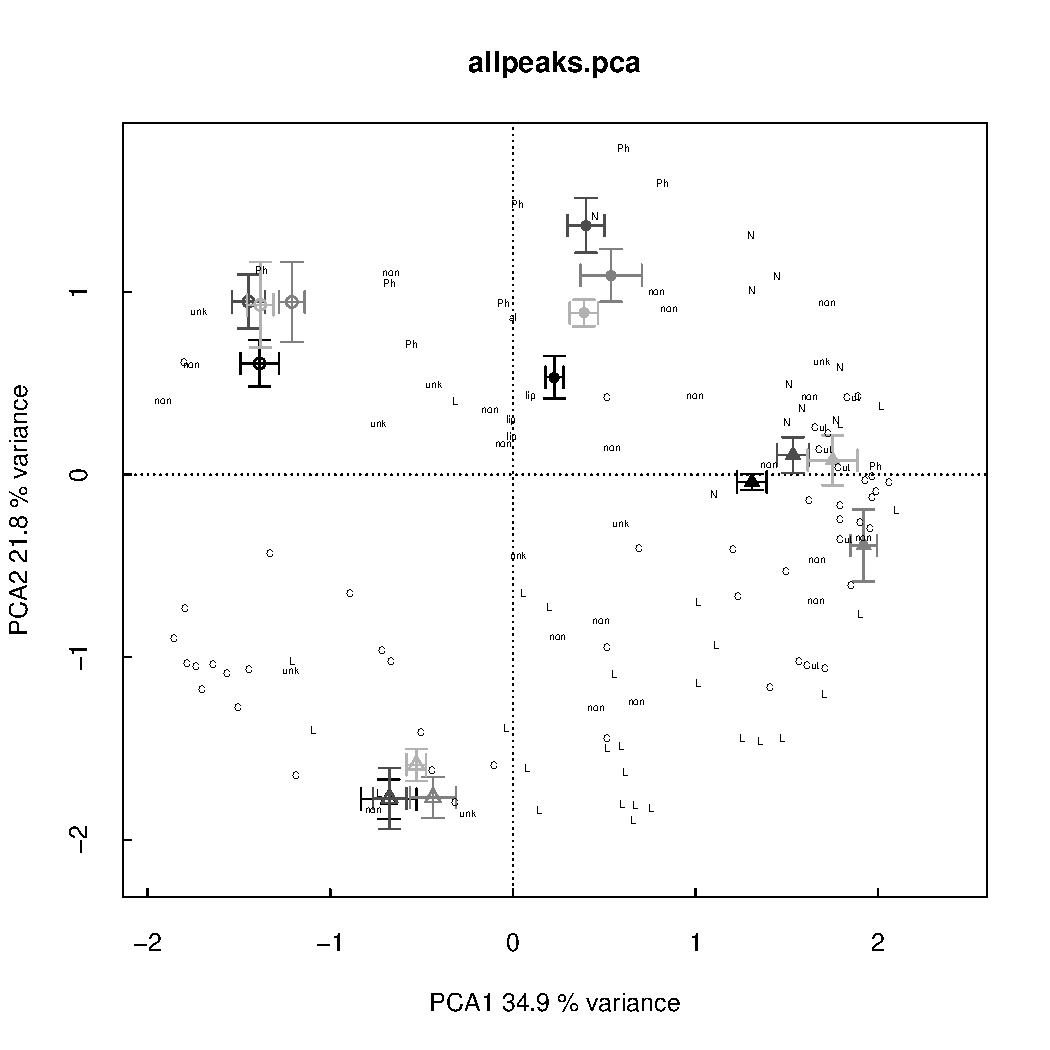
\includegraphics[width=15cm]{allpeaks_PCA12.pdf}
% %\includegraphics[width=10cm]{allpeaks_allharvests_PCA34.pdf}
% \end{center}
\caption{PCA of relative abundances of all 125 pyrolysis products. Open circles - AK, full circles - KL, open triangles - OS, full triangles - SW. black to light grey: harvest 0, 2, 3, and 4. Errorbars indicate 1 SE (n=4-5).}
\label{fig:pca.all}
\end{figure*}


 \newpage
 \begin{figure*}[p]
 \vspace*{2mm}
 %\begin{center}
 %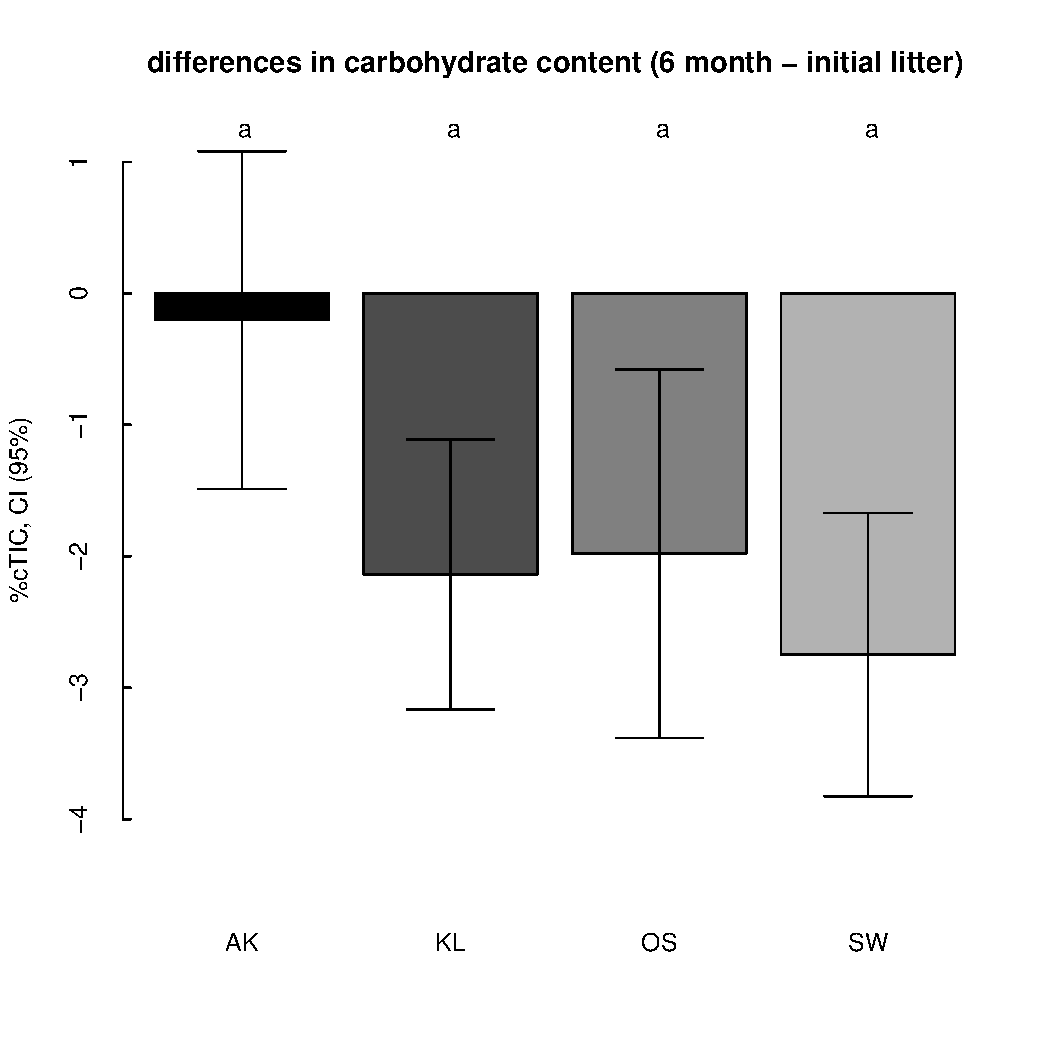
\includegraphics[width=8.3cm]{carb_differences_h3h0.pdf}
 %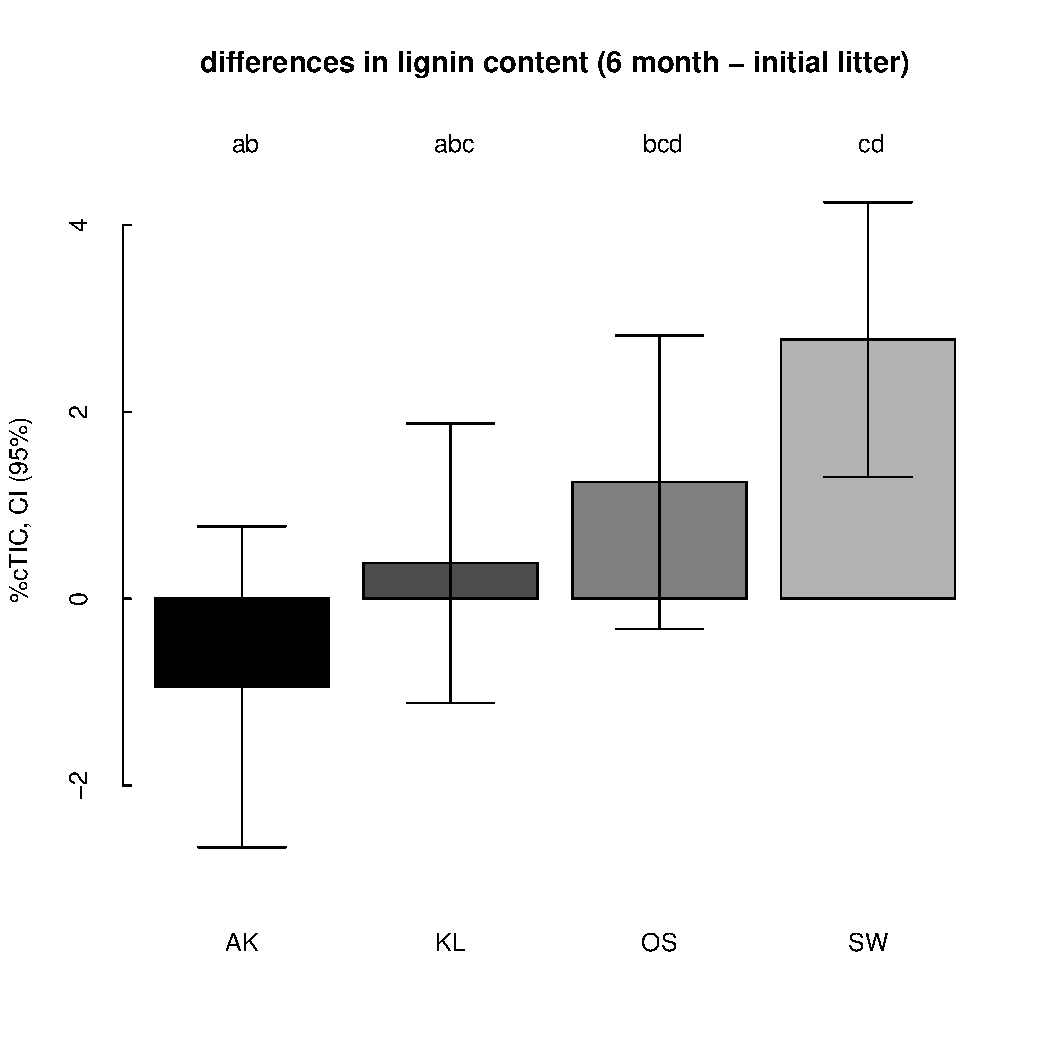
\includegraphics[width=8.3cm]{lig_differences_h3h0.pdf}
 %\end{center}
 \caption{Difference in \% cTIC (sum of lig markers). error bars indicate 95\% confidence intervall.}
 \label{fig:car_lig_6month}
 \end{figure*}


\newpage
\begin{figure*}[p]
\vspace*{2mm}
% \begin{center}
% 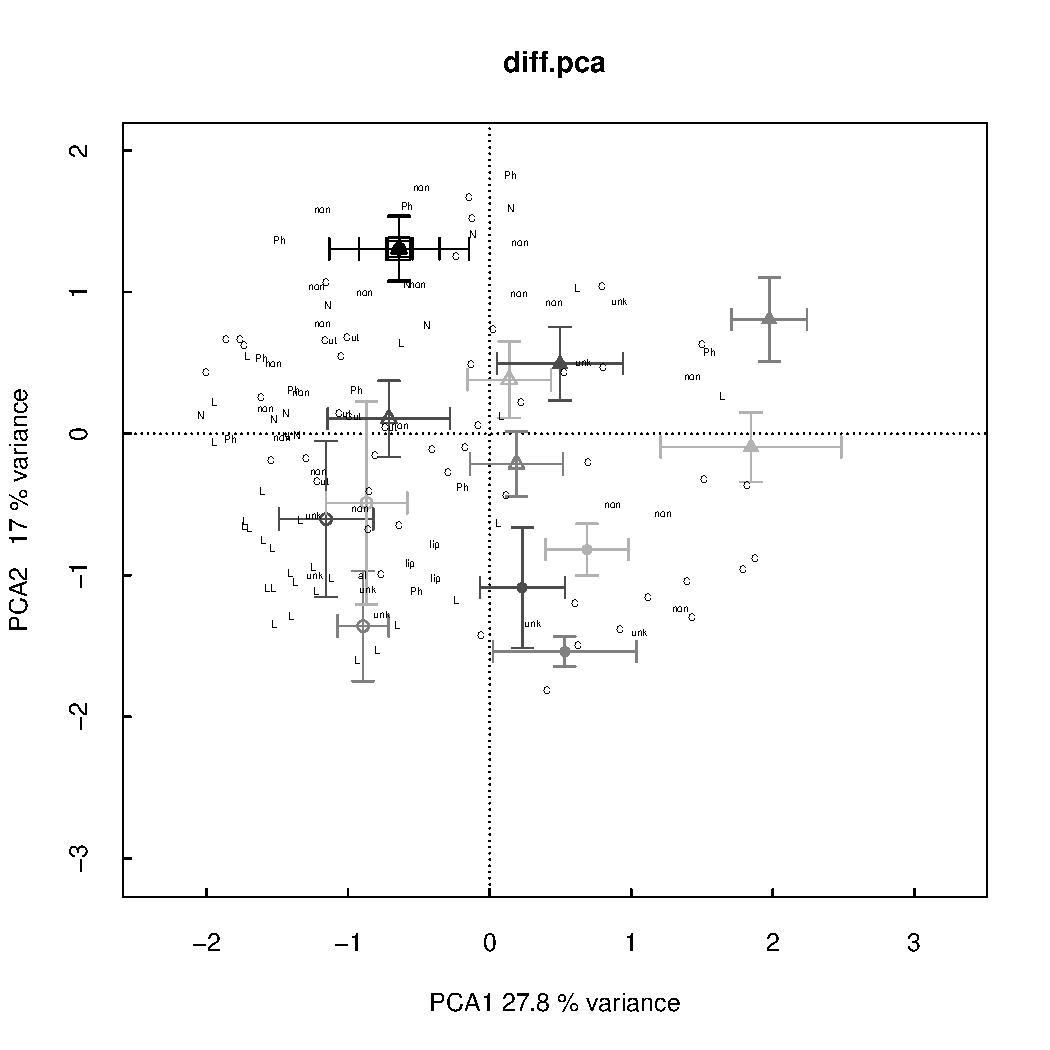
\includegraphics[width=15cm]{allpeaks_diffs_PCA12.pdf}
% \end{center}
\caption{PCA of relative abundances of 125 products minus the mean relative abundance of the product in initial litter of the corresponding litter type. Open circles - AK, full circles - KL, open triangles - OS, full triangles - SW. black to light grey: harvest 0, 2, 3, and 4. Errorbars indicate 1 SE (n=4-5). Decompositino trends follow PCA1 for SW and PCA2 for AK. KL and OS show mixed trends.}
\label{fig:pca.dif}
\end{figure*}


\newpage
\begin{figure*}[p]
\caption{Development of the LCI (Lignin:(Lignin+Carbohydrates) and Lignin:N ratio}
\label{fig:lci}
\end{figure*}


\newpage
\begin{figure*}[p]
\vspace*{2mm}
% \begin{center}
% 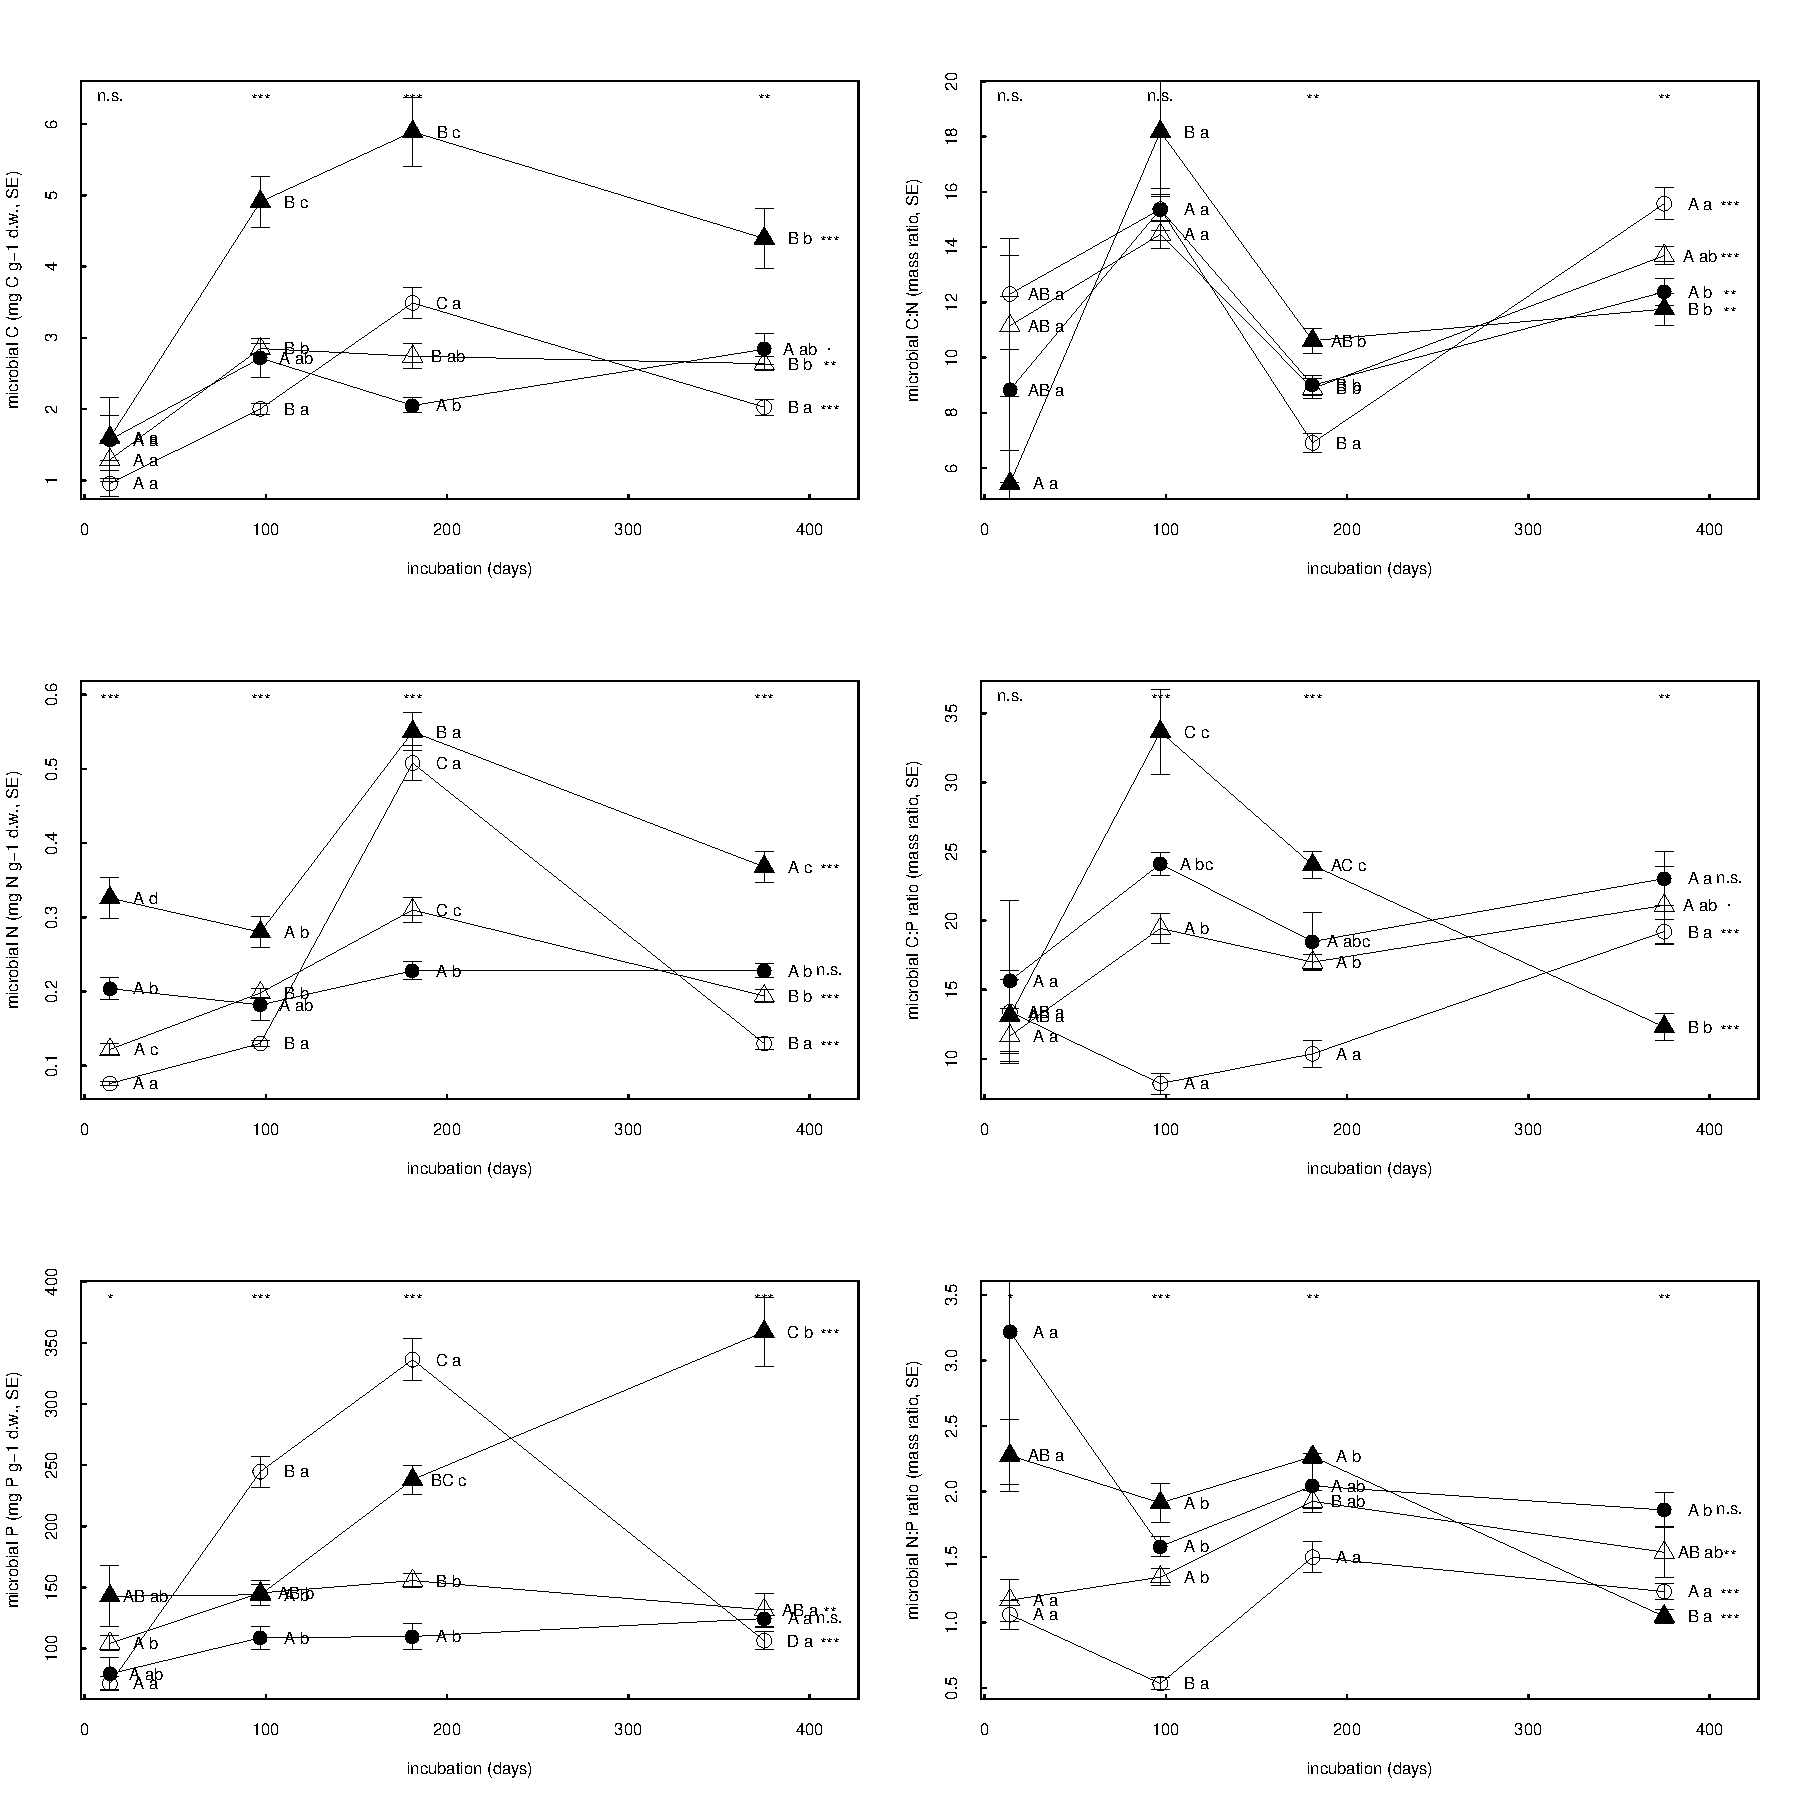
\includegraphics[width=15cm]{microbialbiomass.pdf}
% \end{center}
\caption{Microbial C, N and P content and their ratios.}
\label{fig:bm}
\end{figure*}

\newpage
\begin{figure*}[p]
\vspace*{2mm}
% \begin{center}
% 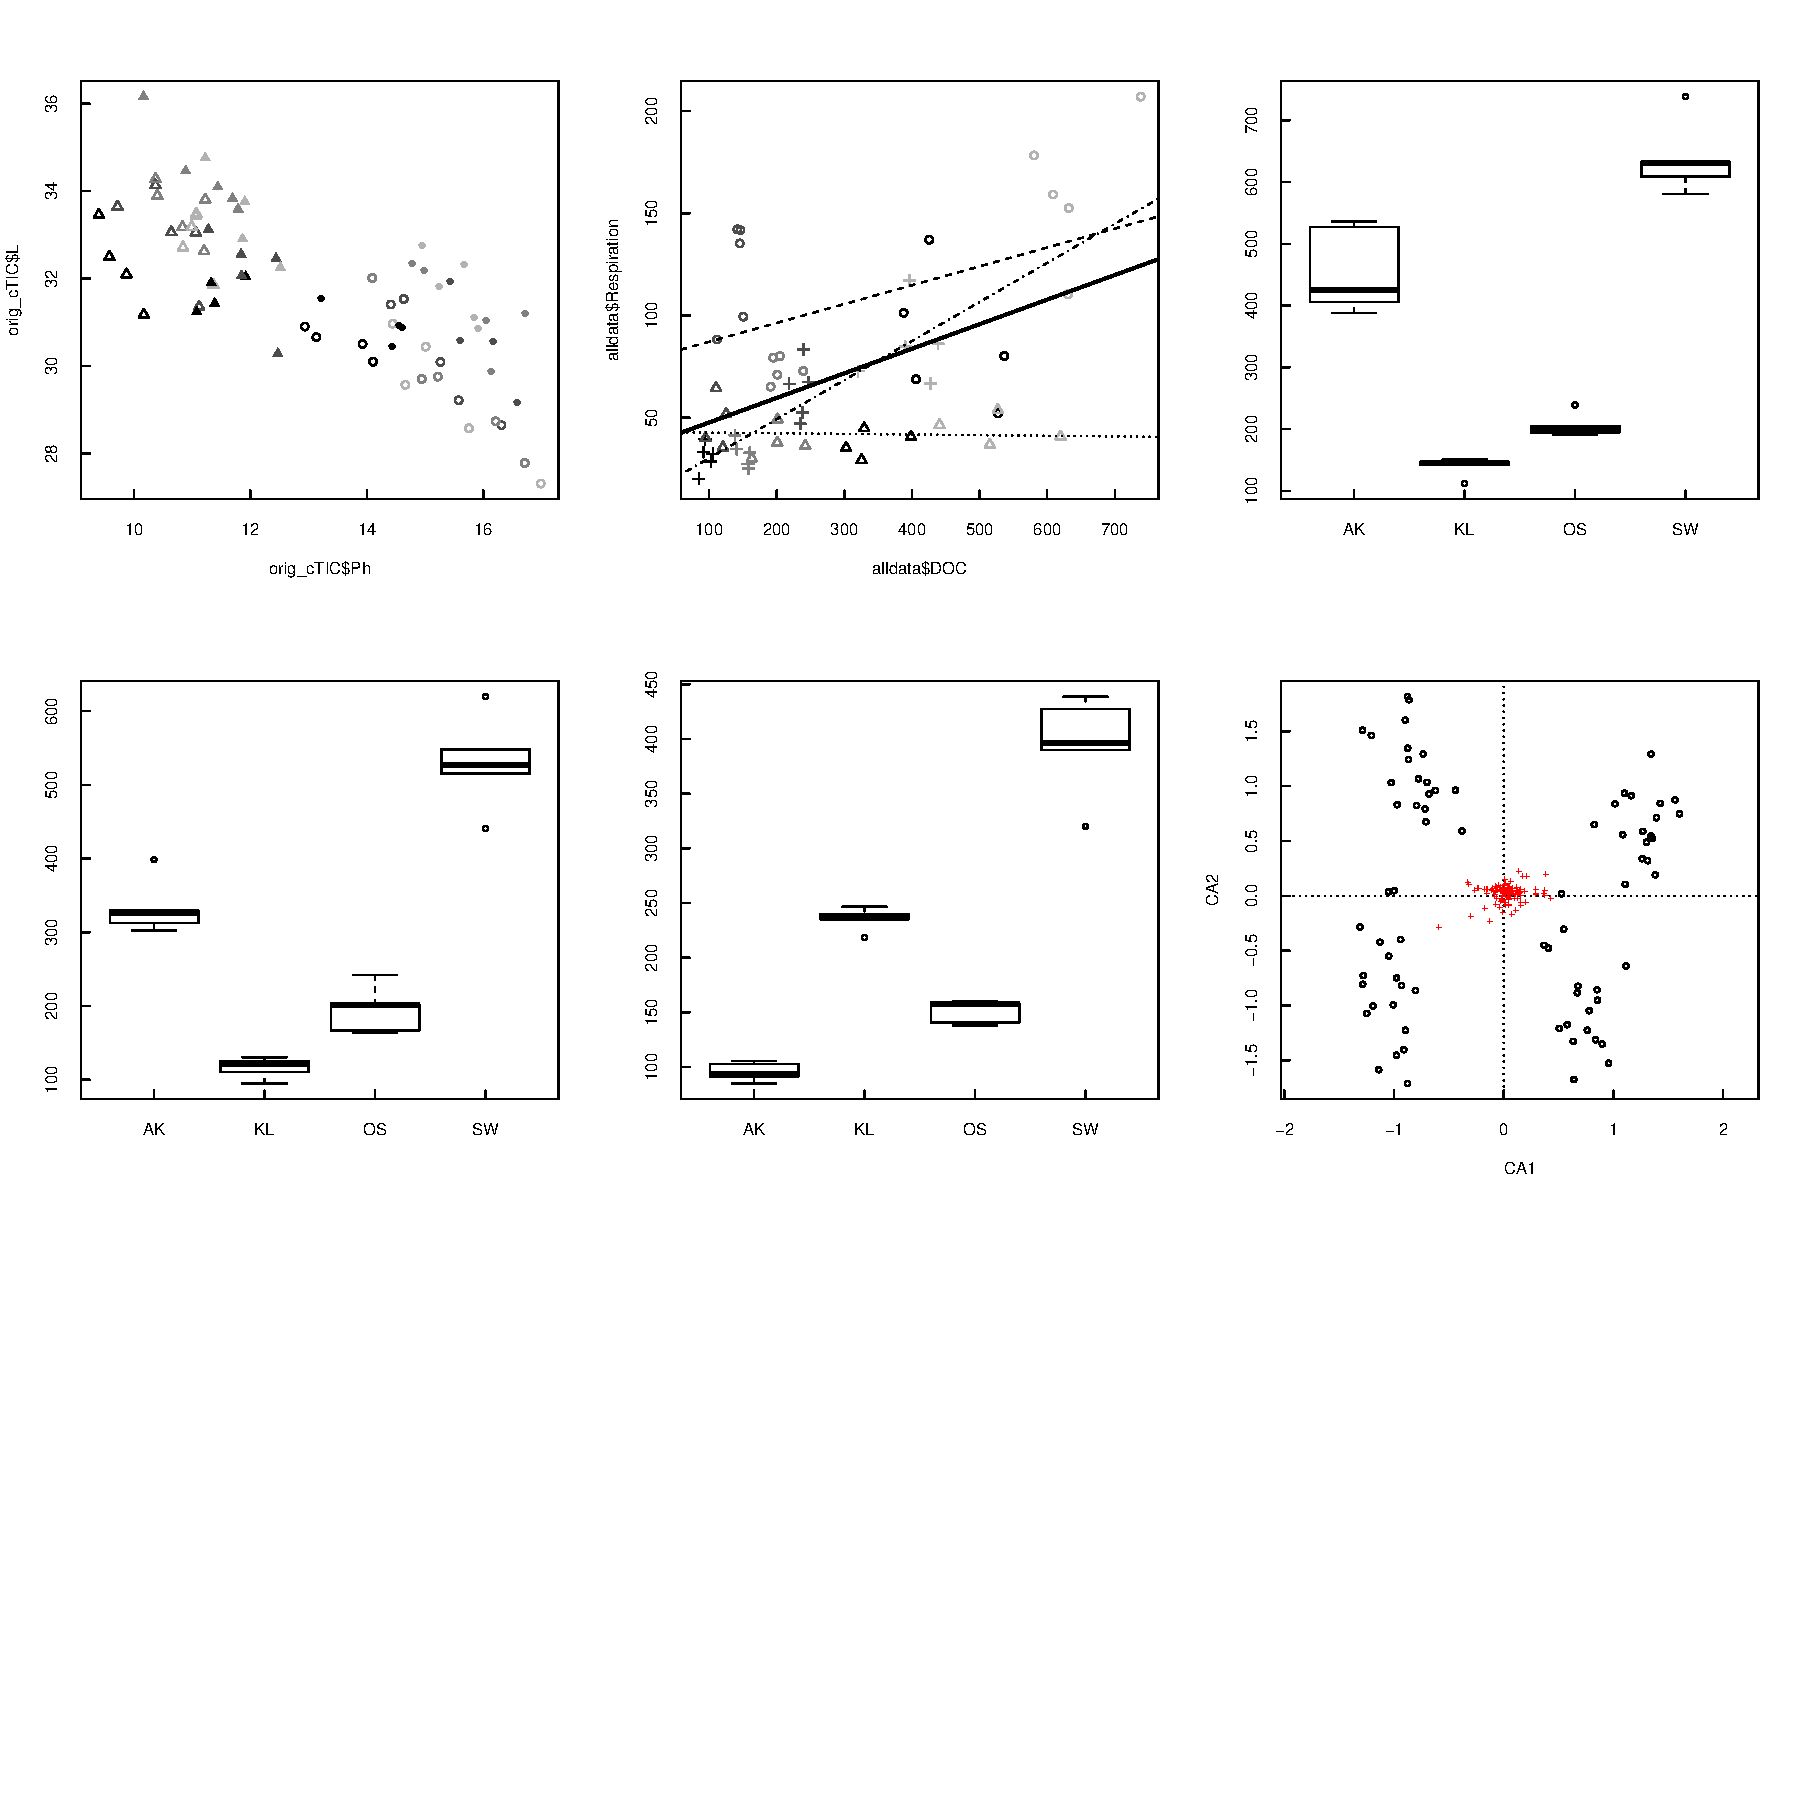
\includegraphics[width=12cm]{enzymes_barplots.pdf}
% \end{center}
\caption{Potential activities of cellulase, phenoloxidase and perodase.}
\label{fig:enz}
\end{figure*}

\newpage
\begin{figure*}[p]
\vspace*{2mm}
% \begin{center}
% 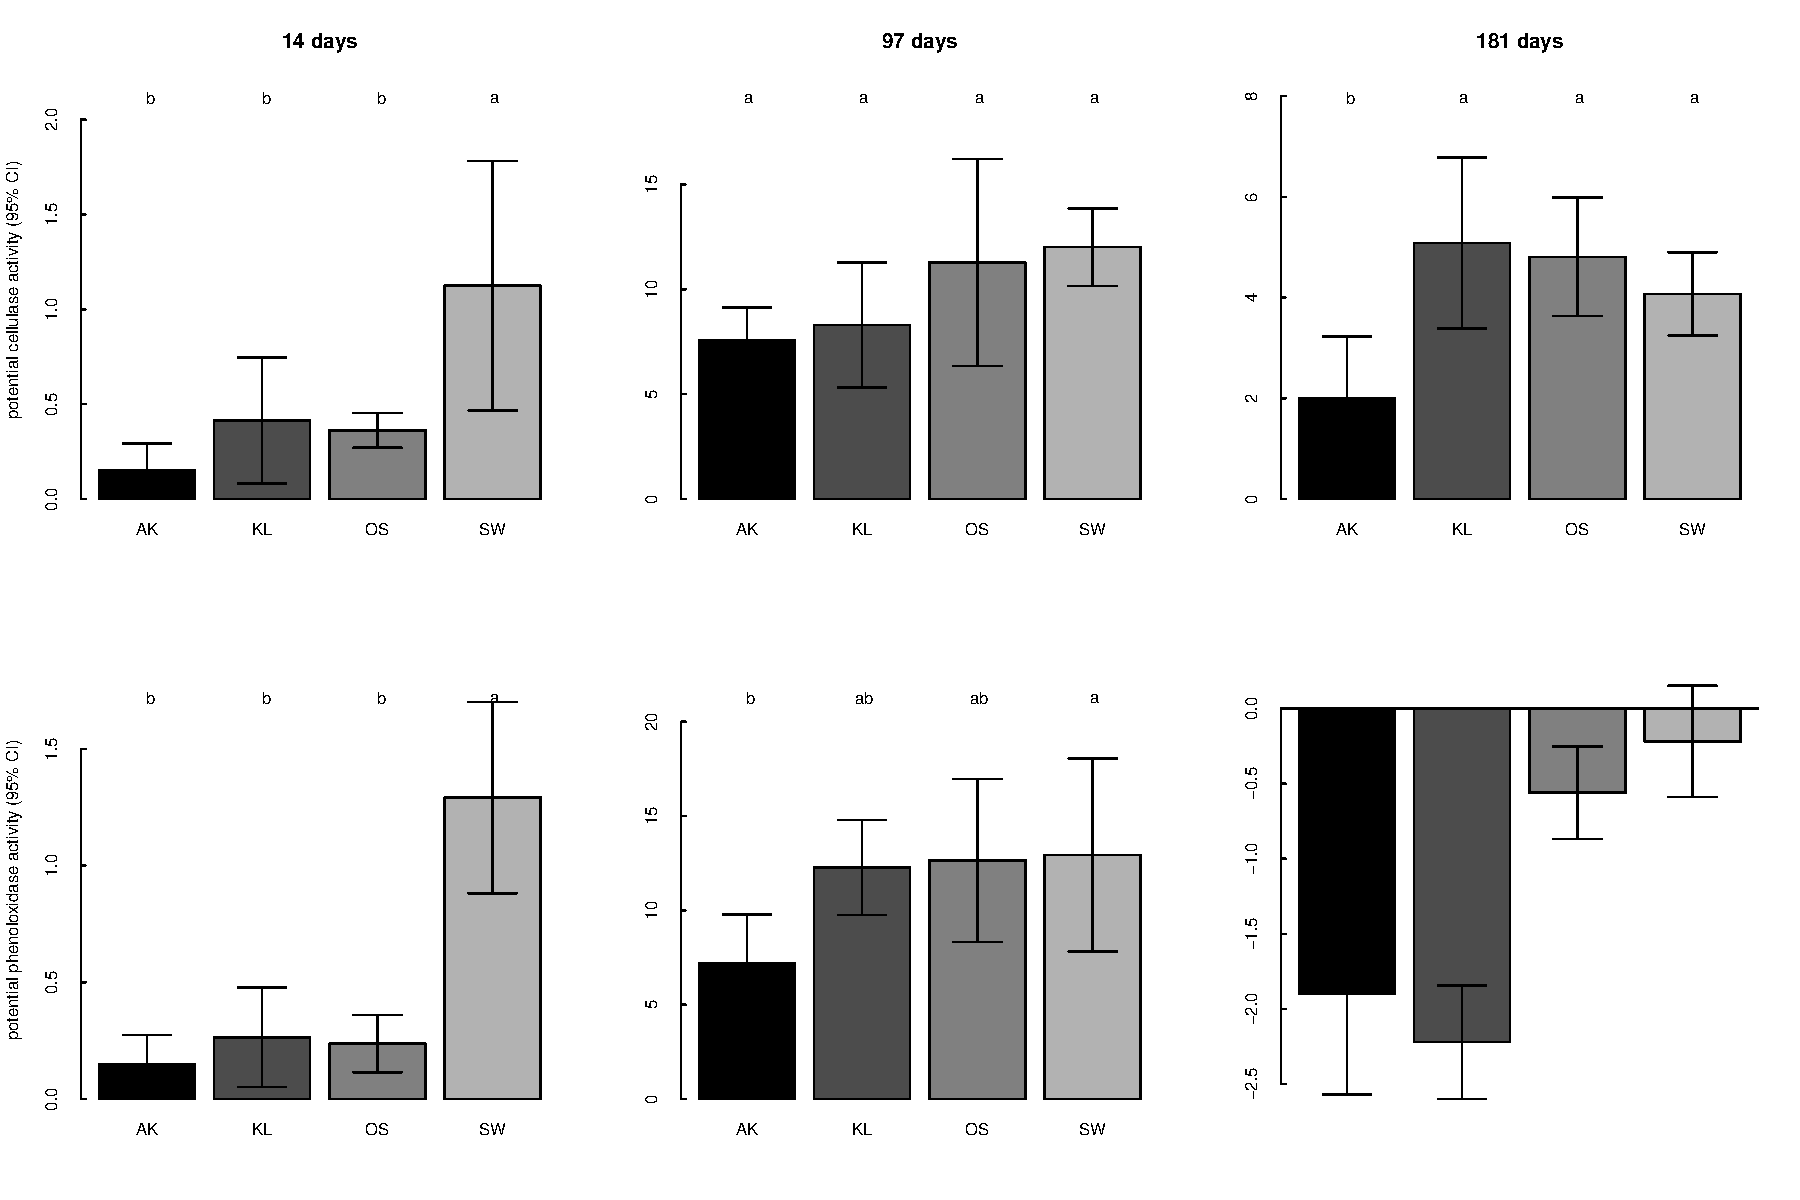
\includegraphics[width=12cm]{enzyme_ratio_barplots.pdf}
% \end{center}
\caption{Ratio between cellulase and two oxidative enzymes (phenolxydase and peroxydase). The two ratios are strongly correlated, oxidative enzymes are higher in AK than in other litter types.}
\label{fig:enz_ratio}
\end{figure*}

\newpage
\begin{figure*}[p]
\vspace*{2mm}
%   \begin{center}
% 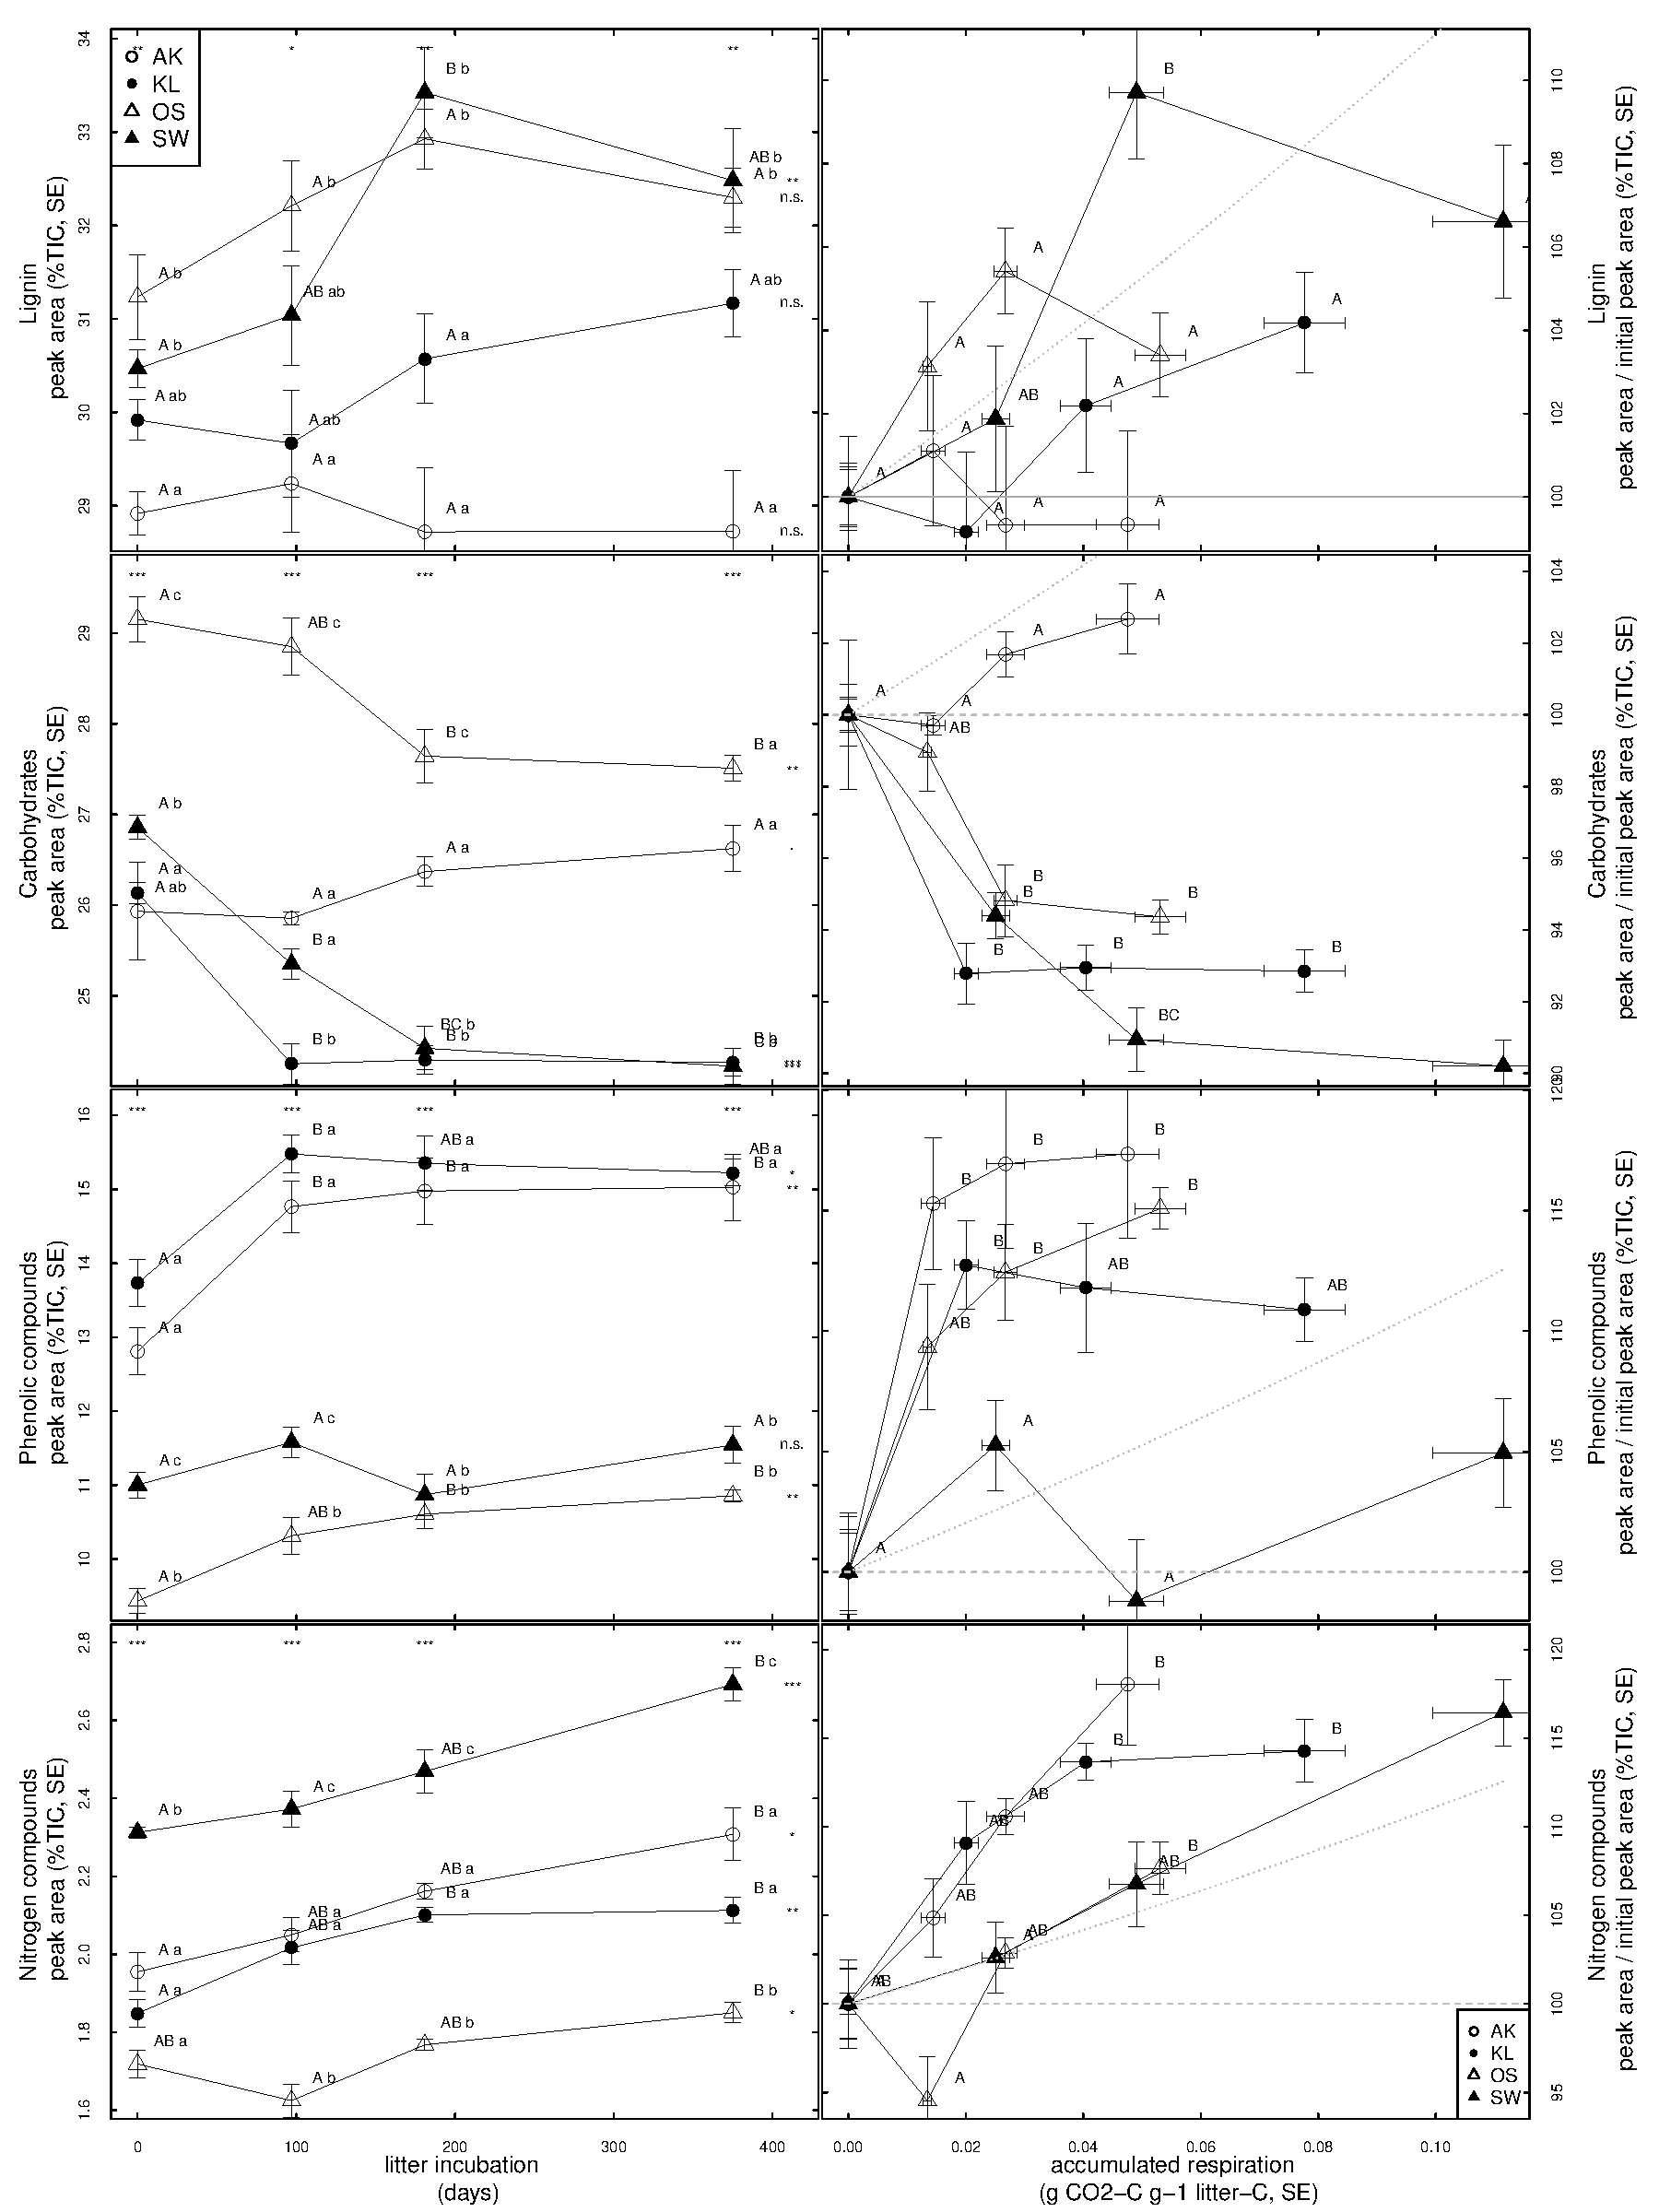
\includegraphics[width=15cm]{timeseries_orig.pdf}
% %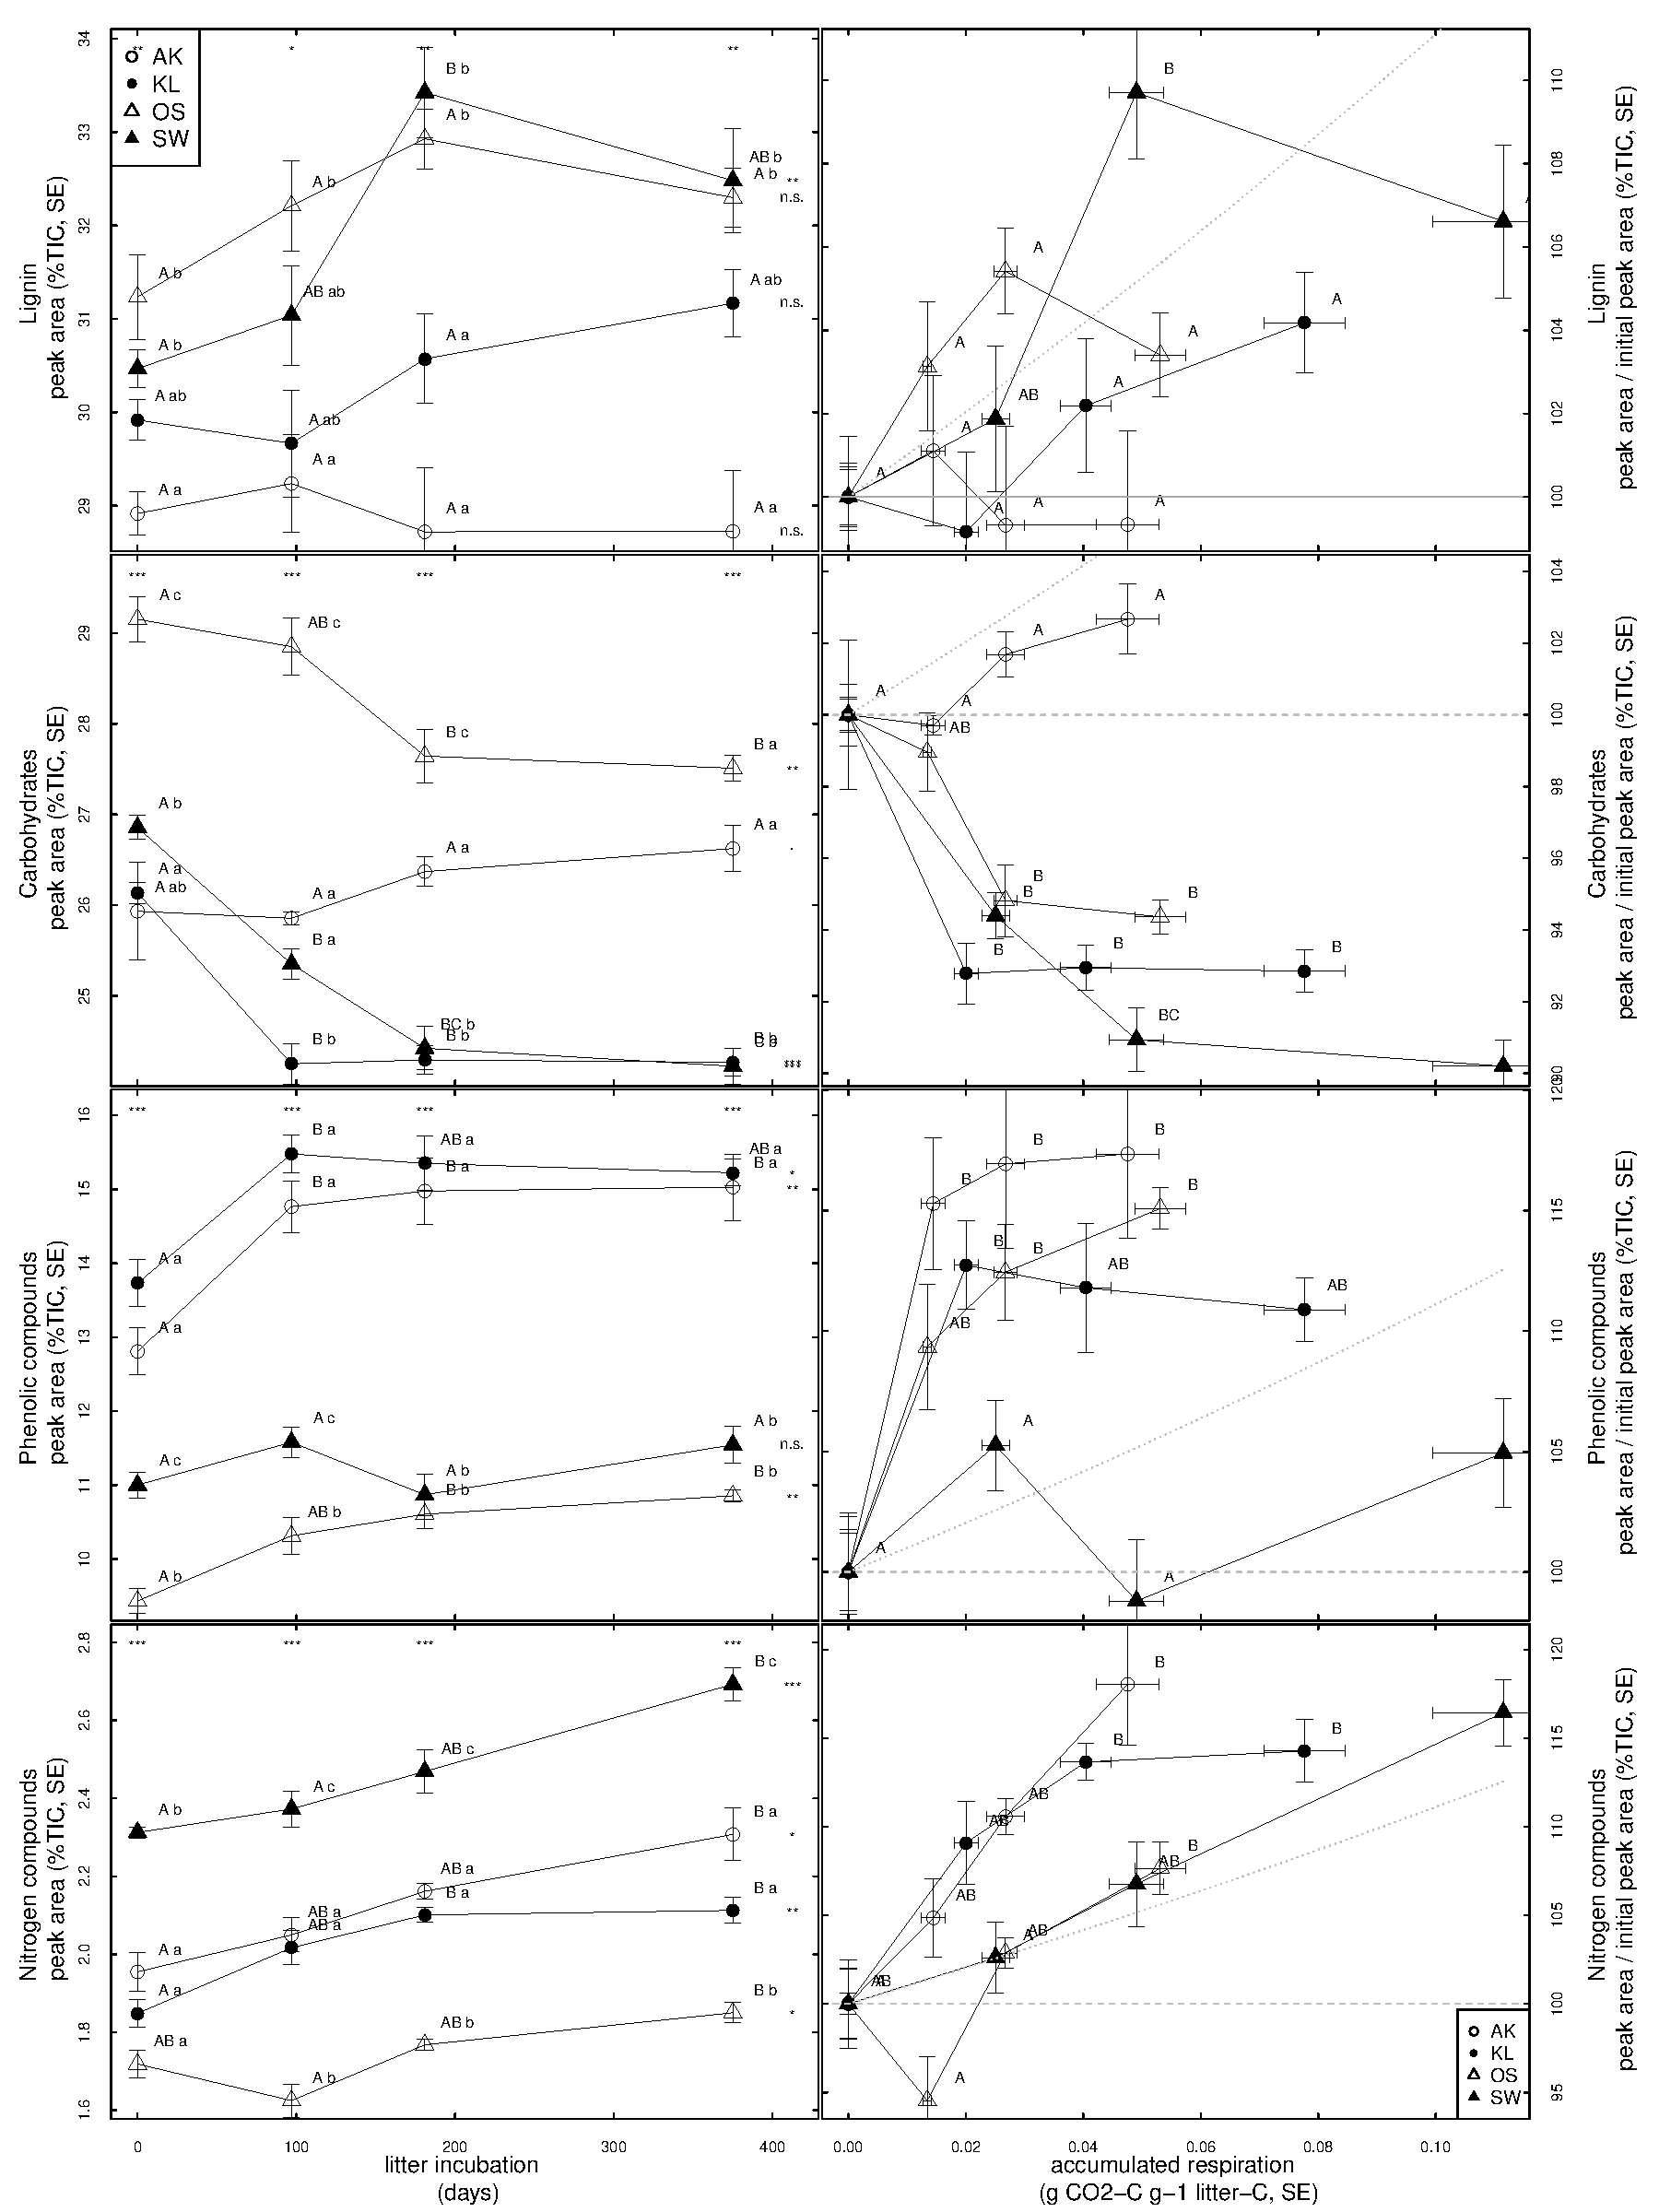
\includegraphics[width=17cm]{timeseries_orig.pdf}
% \end{center}
\caption{Decomposition dynamics of HMW compound classes}
\label{fig:timeseries}
\end{figure*}

\newpage 
\begin{figure*}[p]
\vspace*{2mm}
%   \begin{center}
% 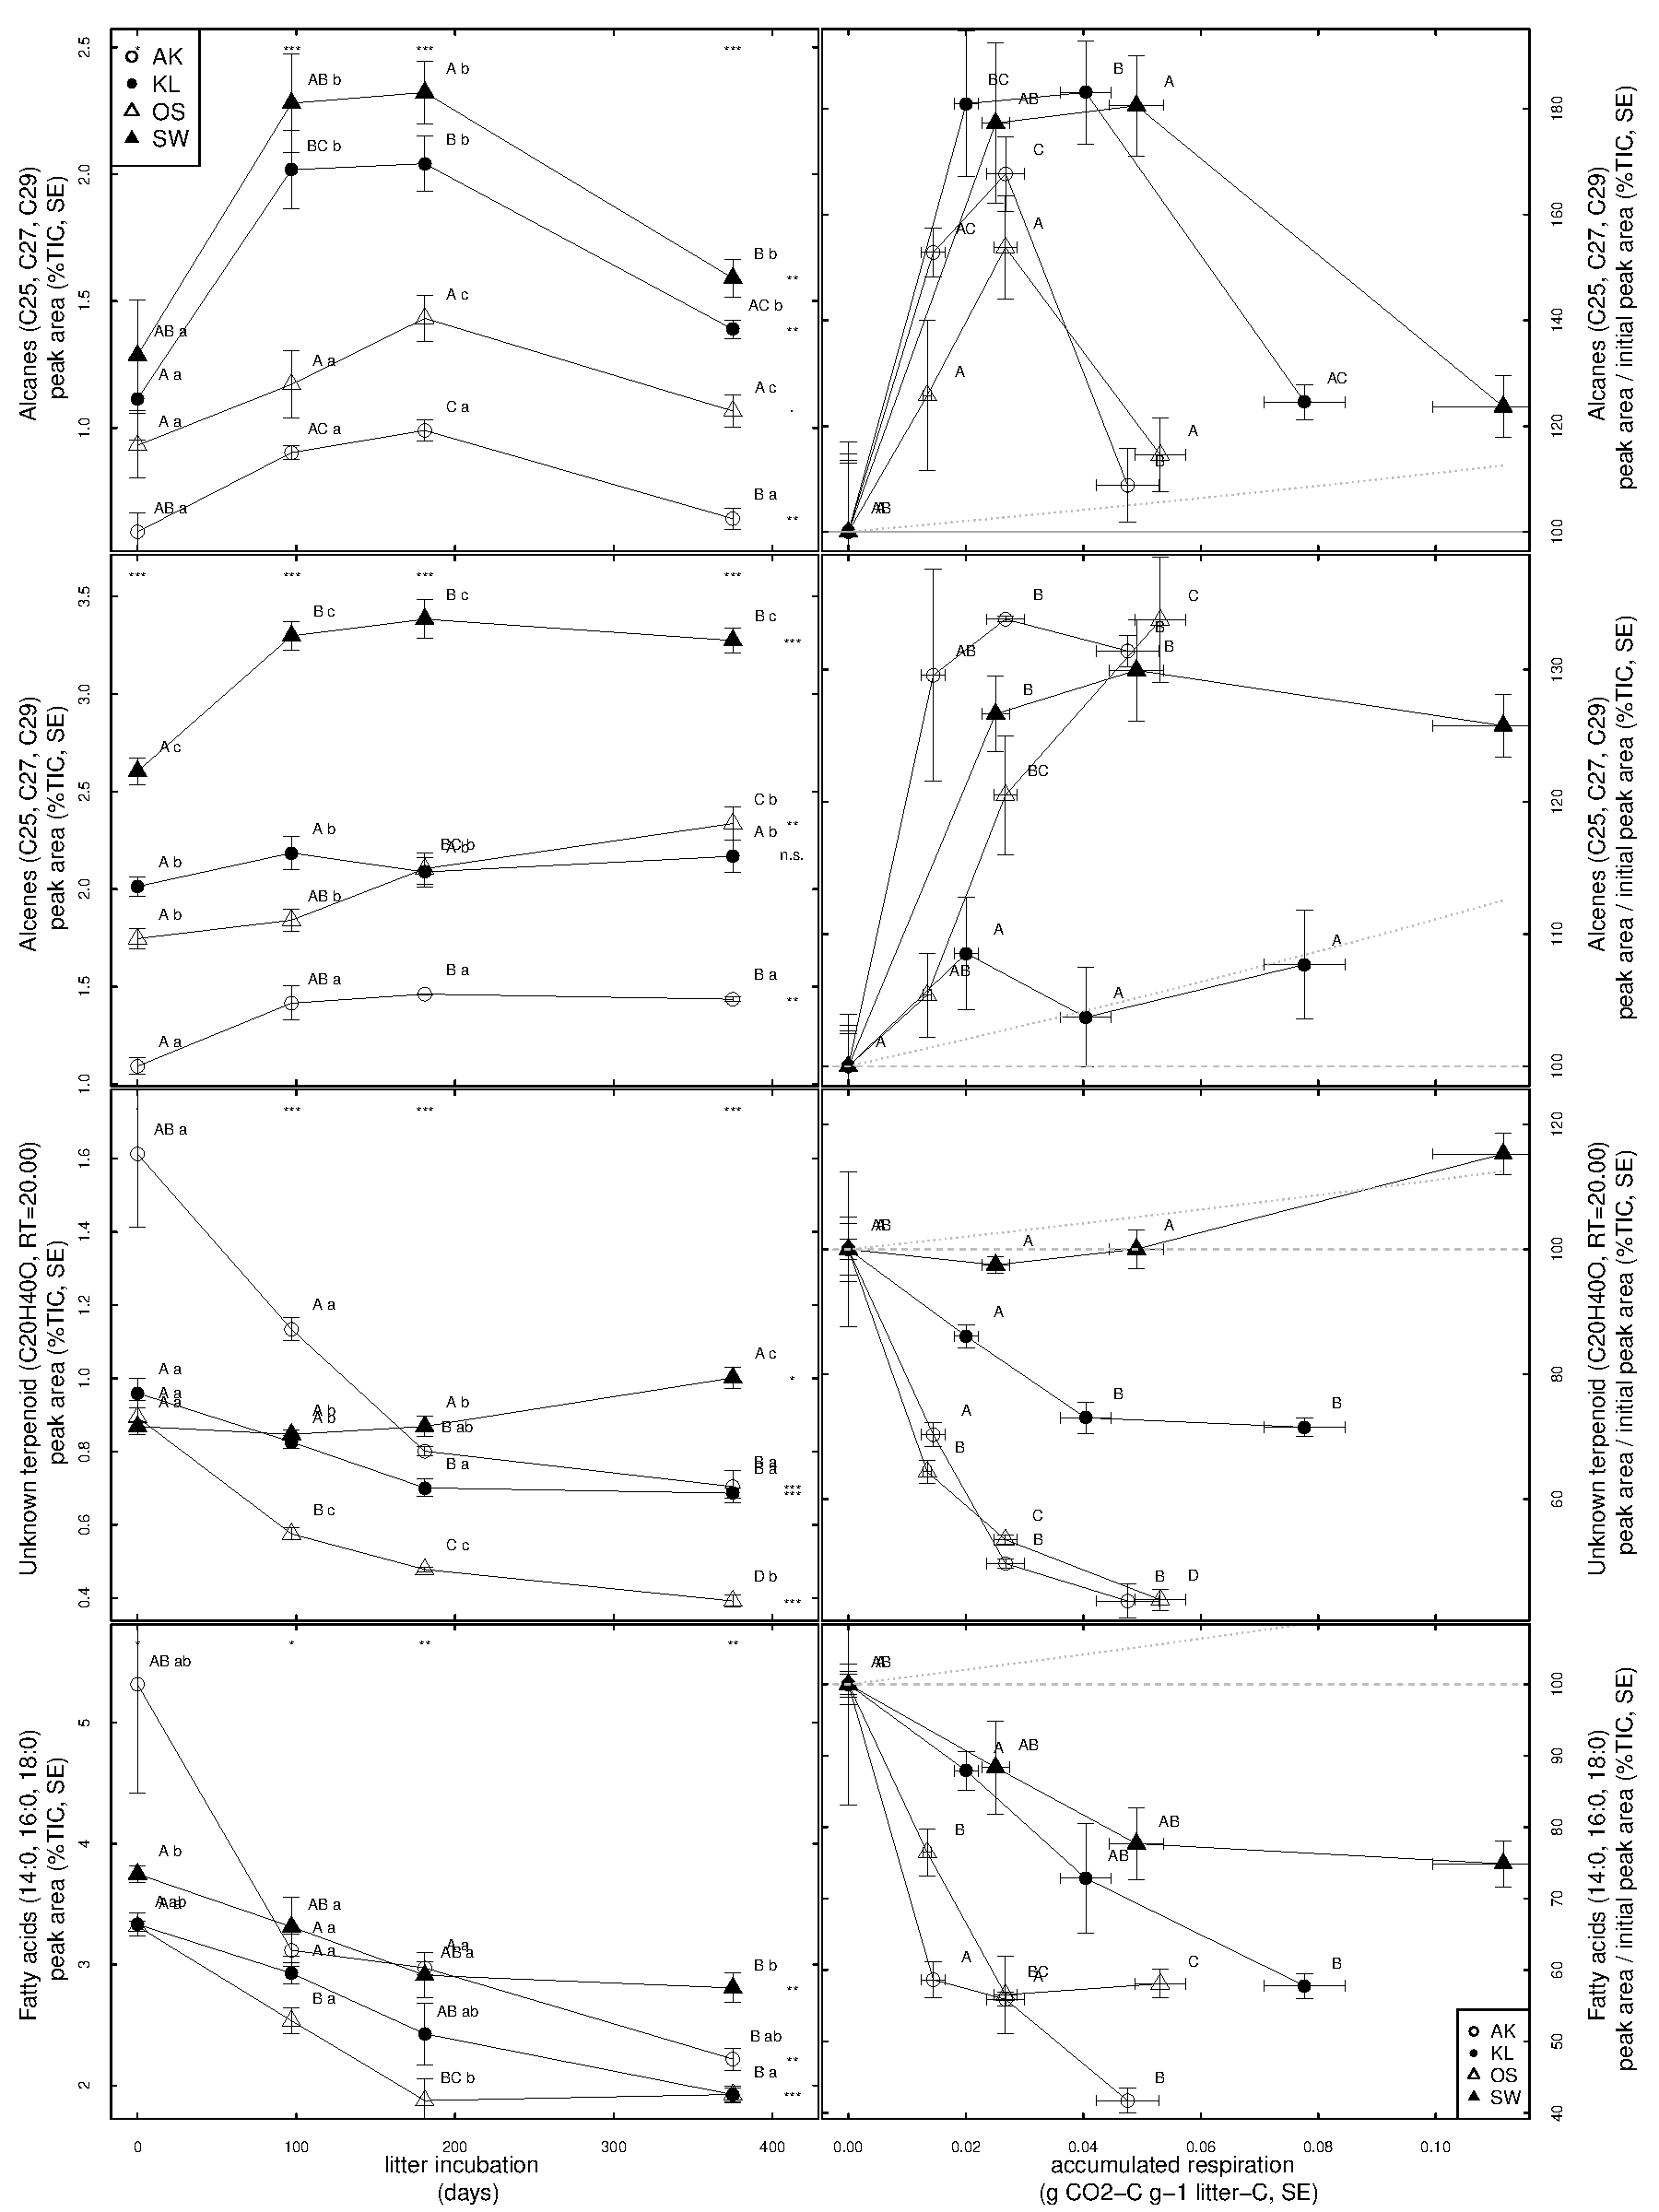
\includegraphics[width=15cm]{timeseries_waxes.pdf}
% %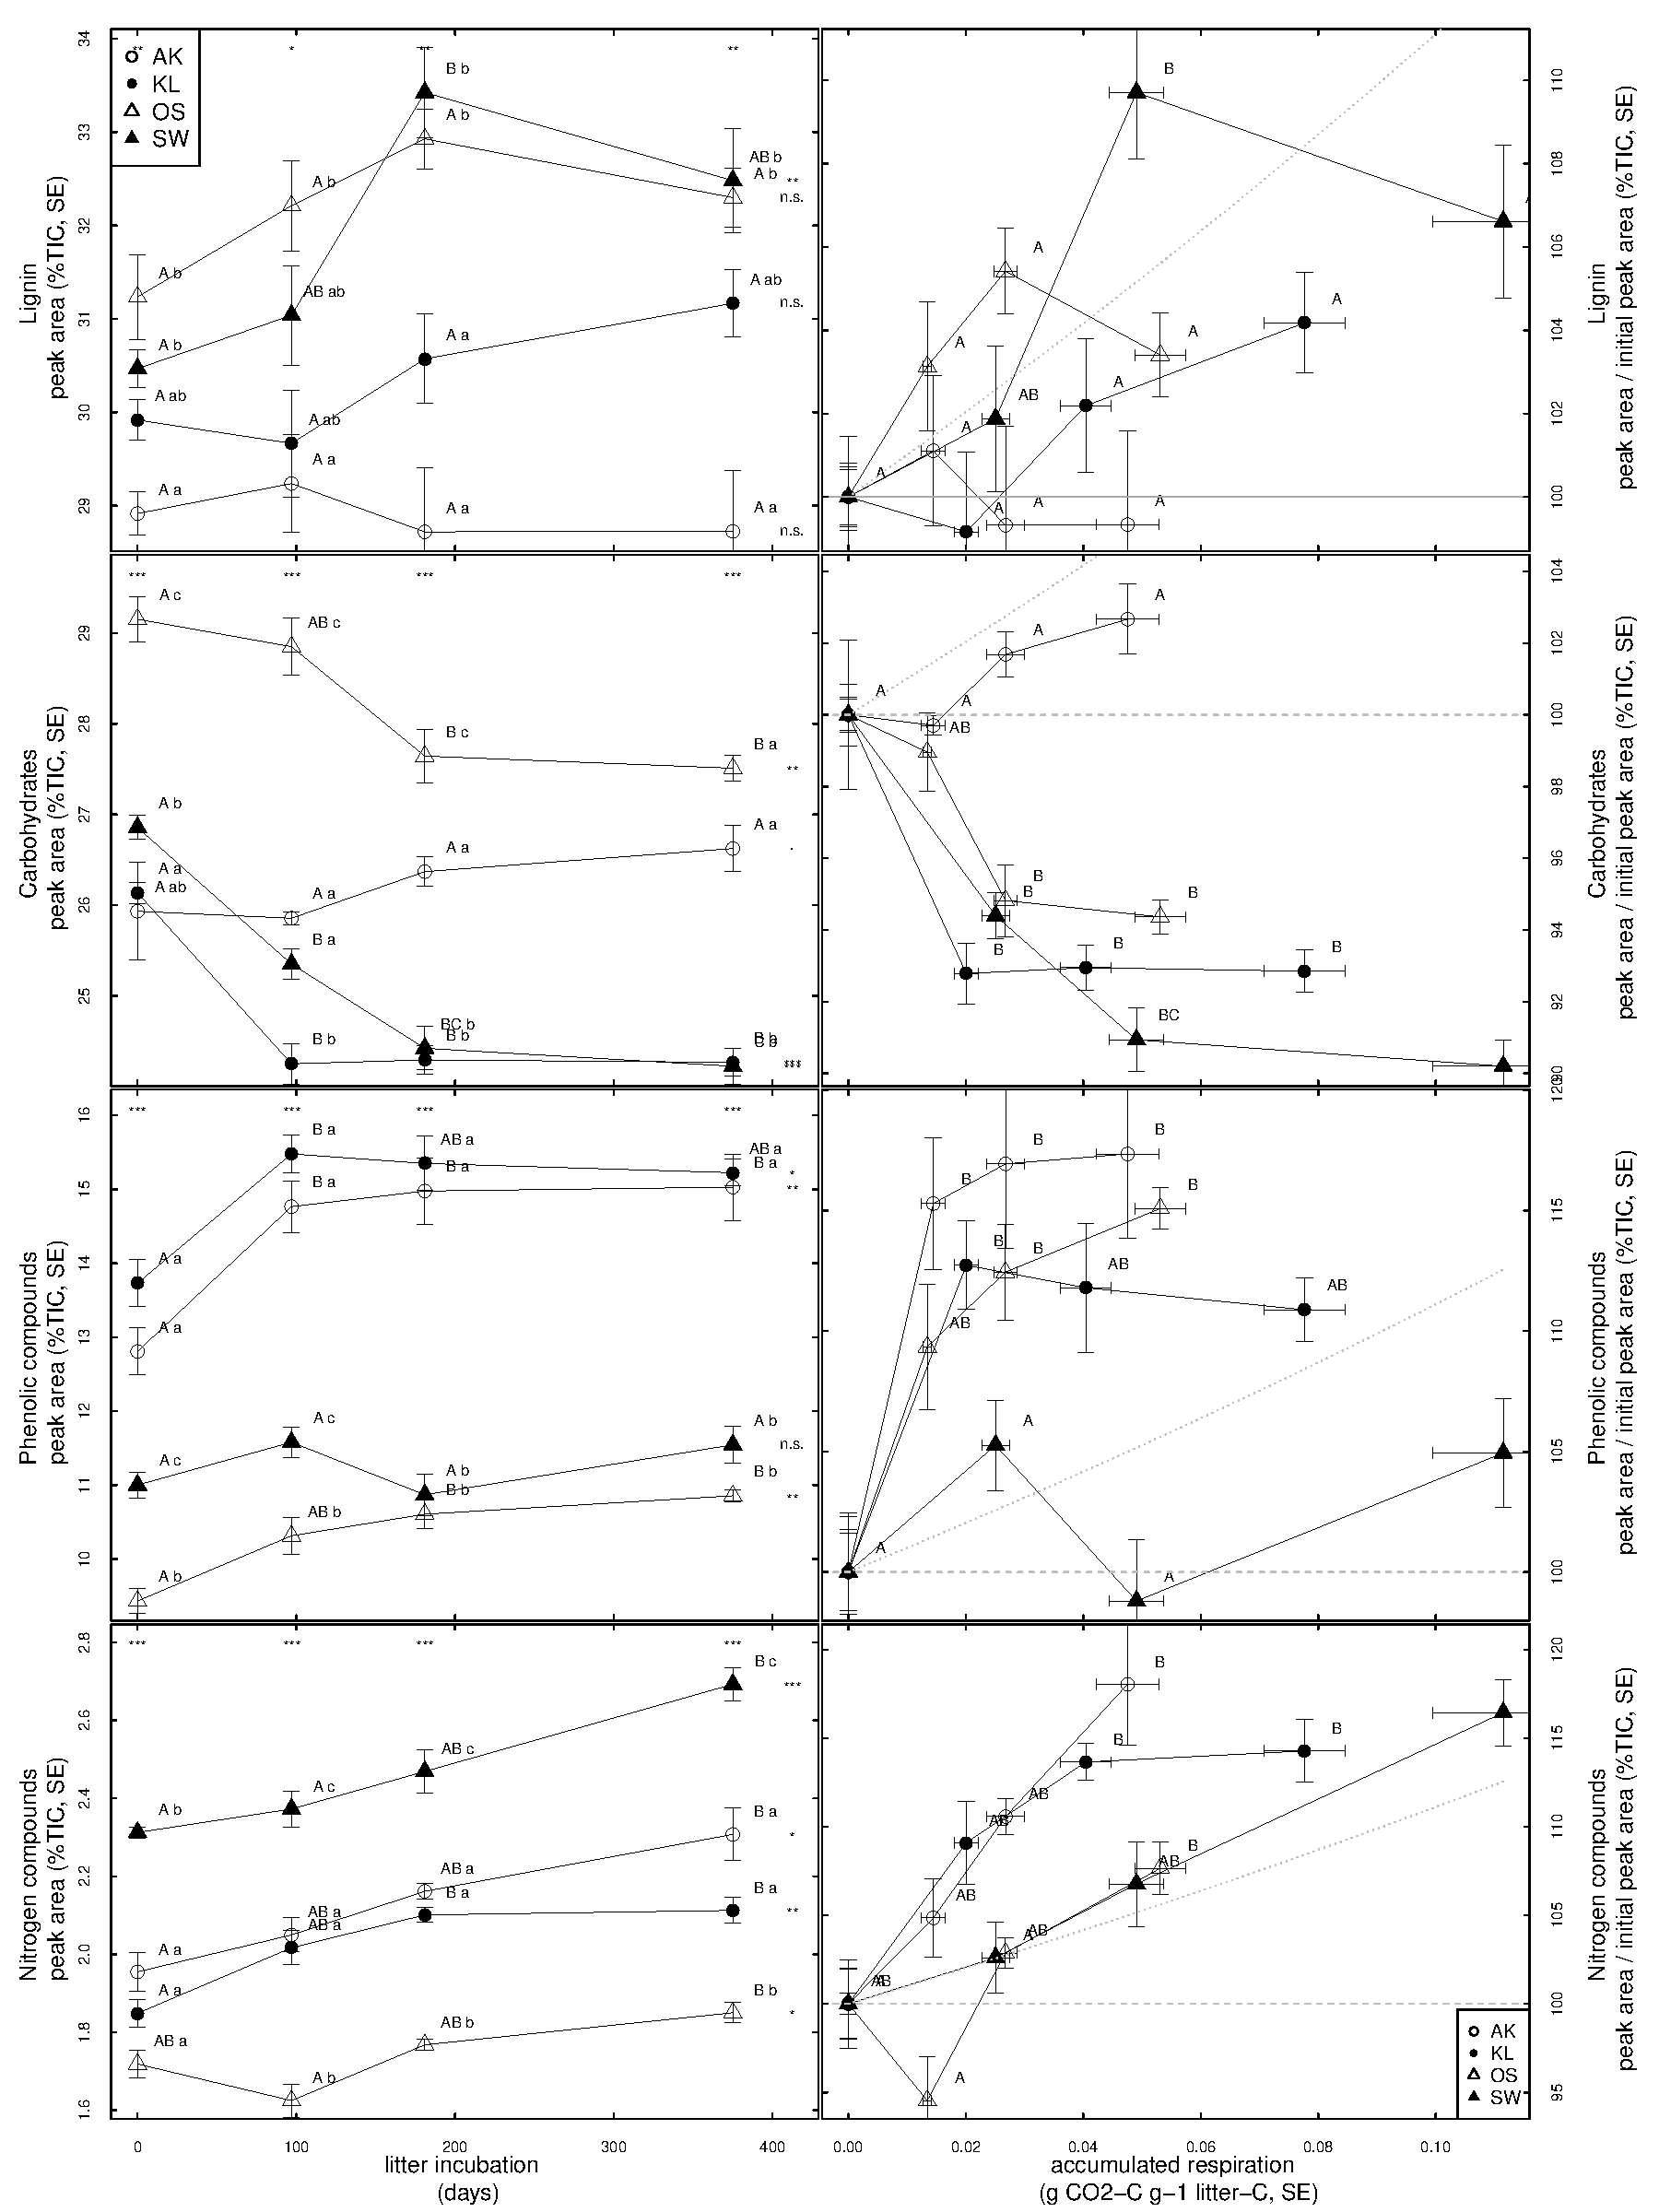
\includegraphics[width=17cm]{timeseries_orig.pdf}
% \end{center}
\caption{Decomposition dynamics of lipophilic compound classes}
\label{fig:waxes}
\end{figure*}





% \begin{figure*}[p]
% \vspace*{2mm}
% \begin{center}
% 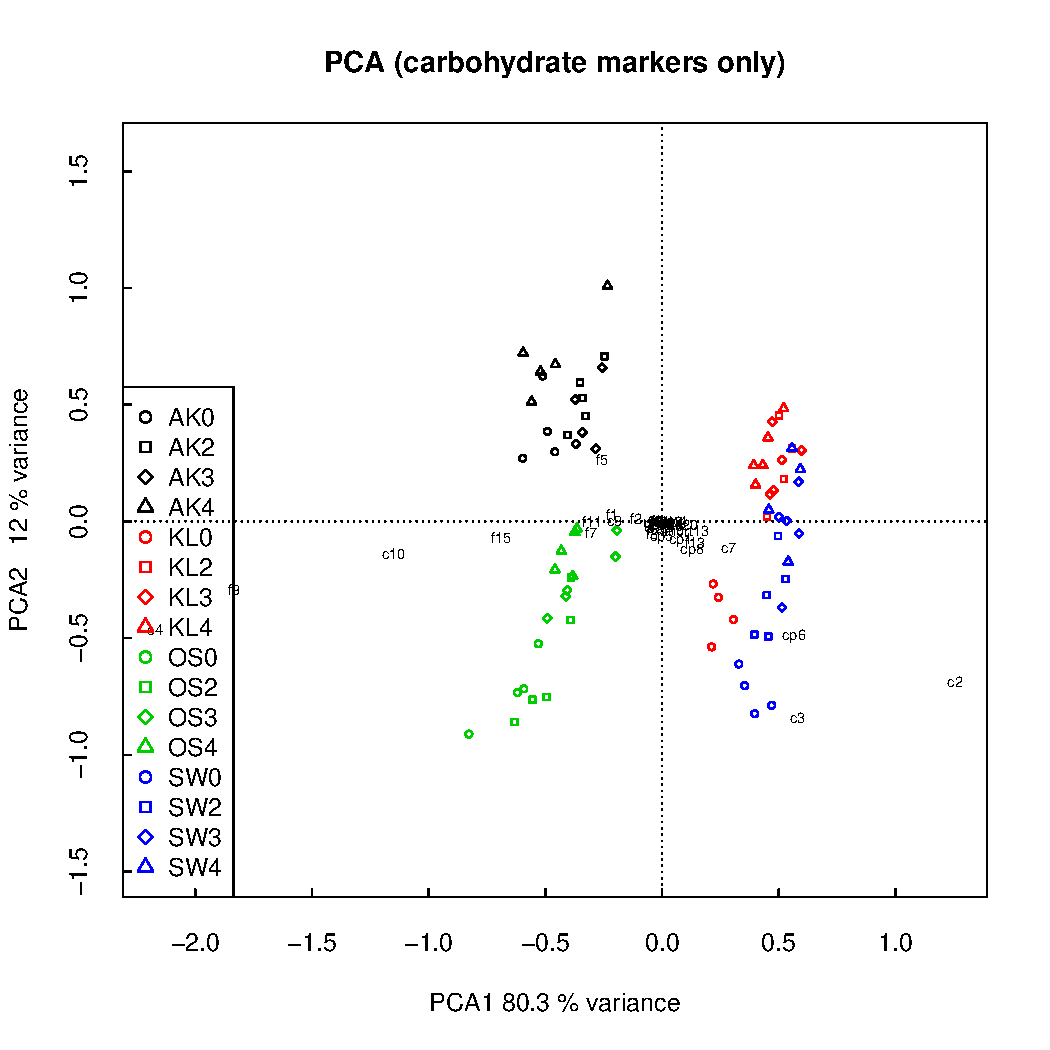
\includegraphics[width=10cm]{pca12_carbos.pdf}
% 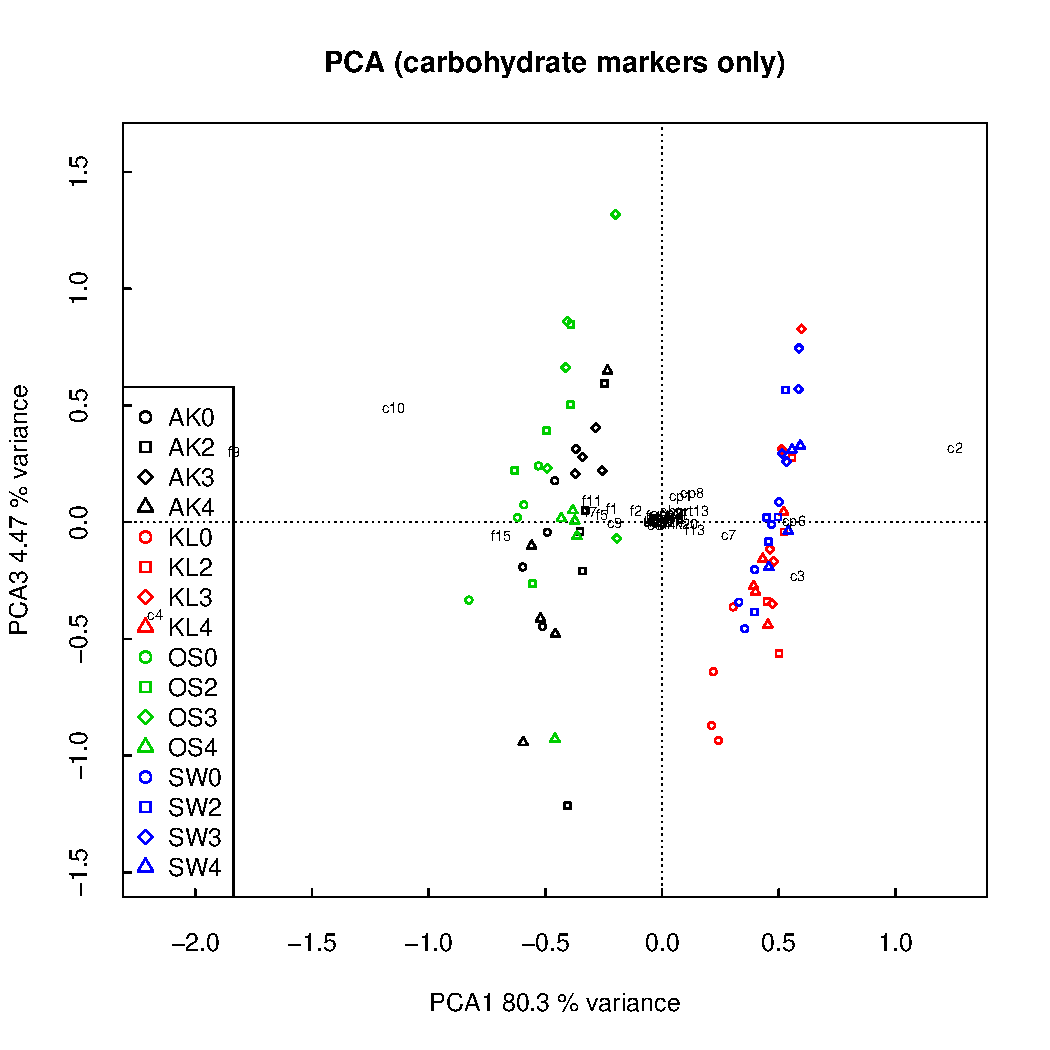
\includegraphics[width=10cm]{pca13_carbos.pdf}
% 
% \end{center}
% \caption{TEXT}
% \end{figure*}
% 
% %% TWO-COLUMN FIGURES
% 
% %f
% \begin{figure*}[p]
% \vspace*{2mm}
% \begin{center}
% \includegraphics[width=10cm]{ligonly_allharvests_PCA12.pdf}
% 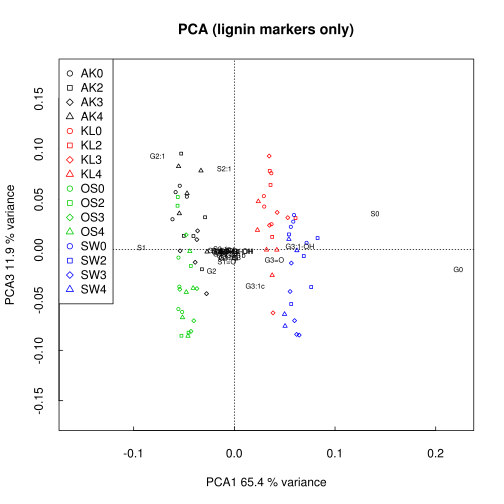
\includegraphics[width=10cm]{ligonly_allharvests_PCA13.pdf}
% \end{center}
% \caption{TEXT}
% \end{figure*}
% 

\newpage
 \begin{figure*}[p]
%  \vspace*{2mm}
%  \begin{center}
%  \includegraphics[width=15cm]{controls_h1.pdf}
%  \end{center}
 \caption{Litter chemistry: content of macro and micronutrients, 14 days after innoculation, n=5}
 \label{fig:litchem_h1}
 \end{figure*}

% \begin{figure*}[p]
% \vspace*{2mm}
% \begin{center}
% \includegraphics[width=12cm]{controls_h2.pdf}
% \end{center}
% \caption{Litter chemistry: content of macro and micronutrients, 97 days after innoculation, n=5}
% \label{fig:litchem_h2}
% \end{figure*}

\newpage
\begin{figure*}[p]
%\vspace*{2mm}
% \begin{center}
% 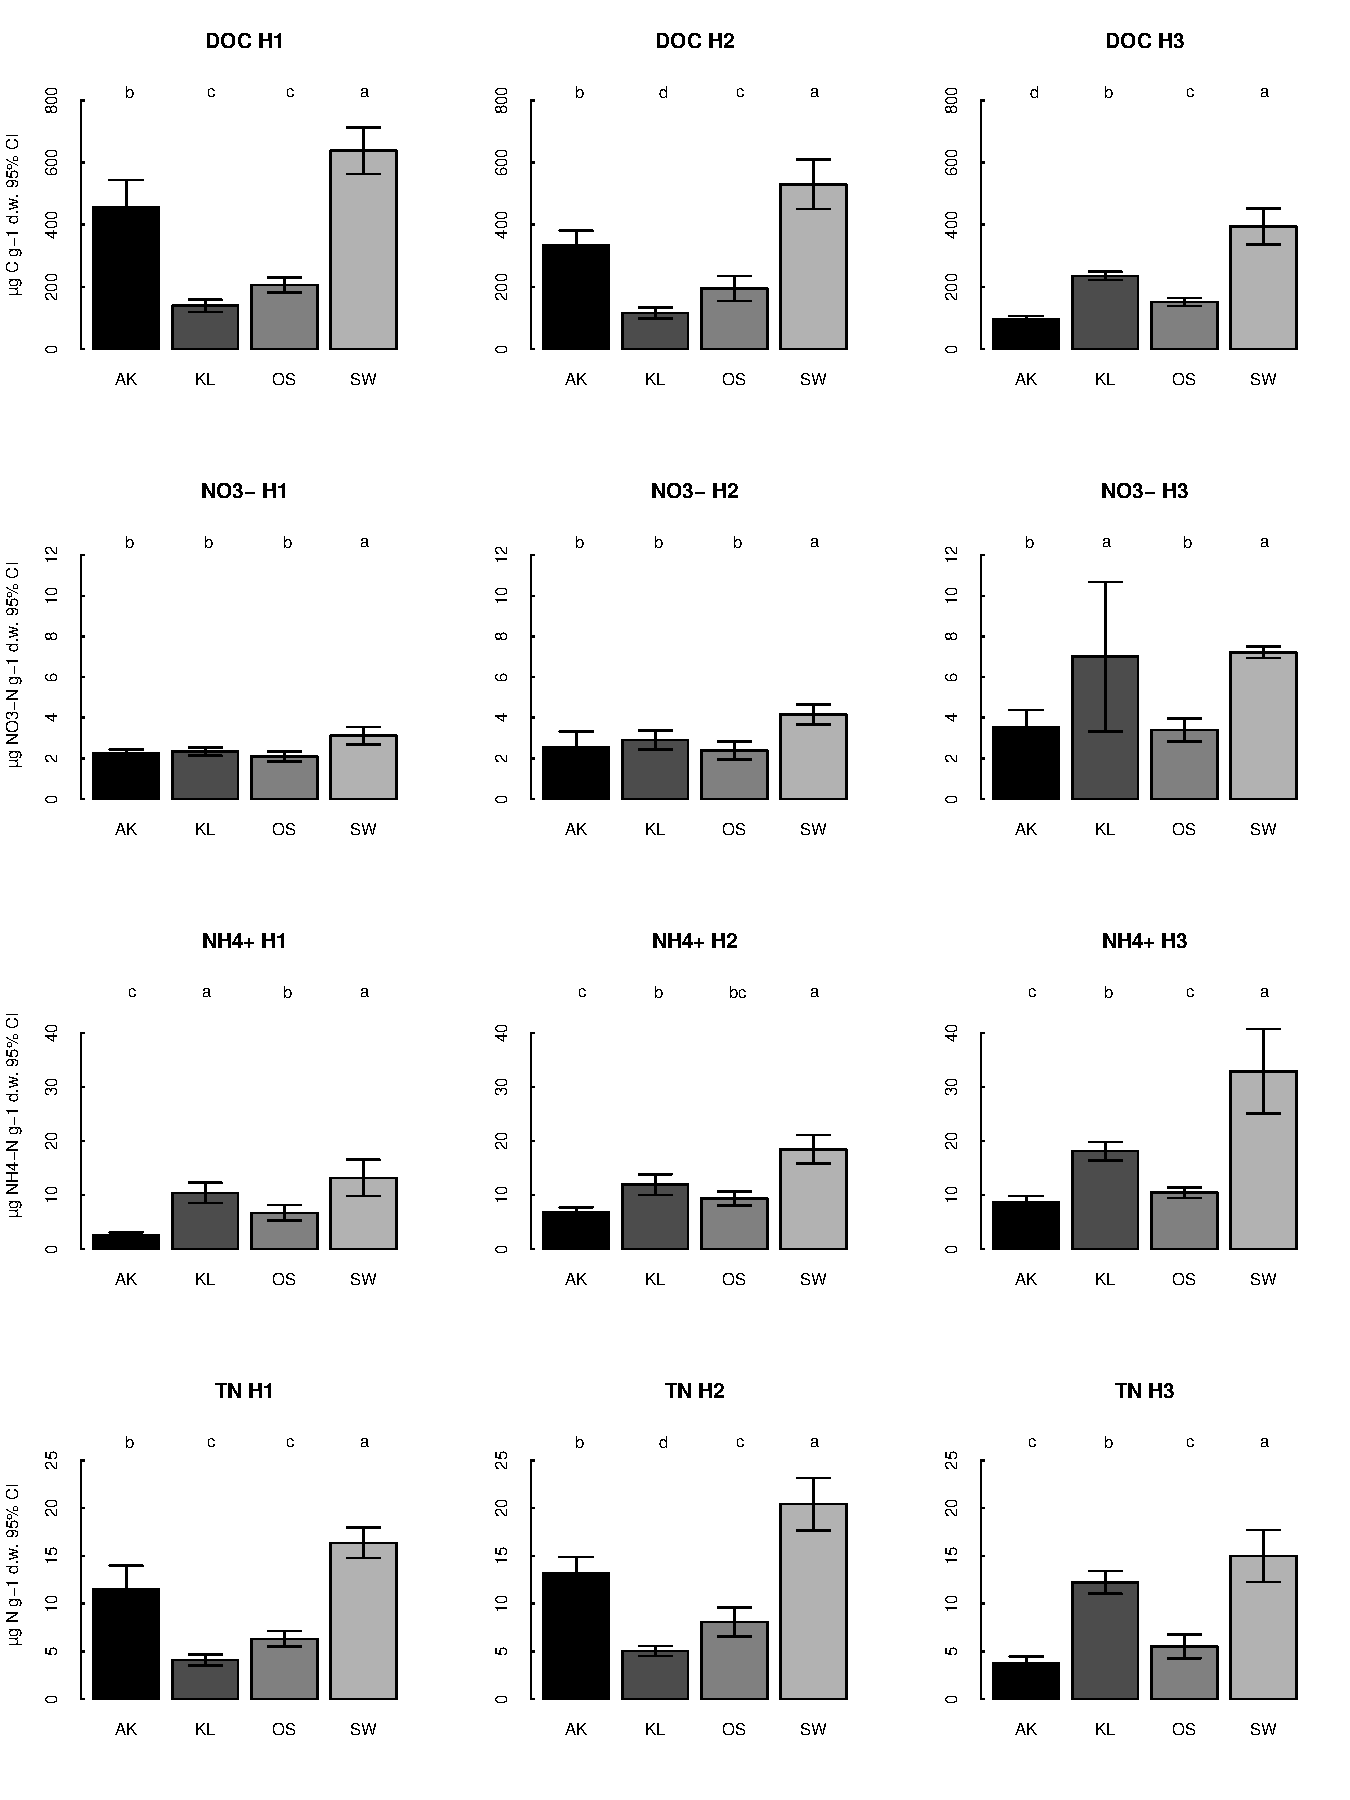
\includegraphics[width=15cm]{doc_barplots.pdf}
% \end{center}
\caption{Litter Chemistry: Dissolved organic carbon, total dissolved nitrogen, NO3-, NH4+}
\label{fig:doc}
\end{figure*}

% \newpage
% \begin{figure*}[p]
% \vspace*{2mm}
% \begin{center}
% 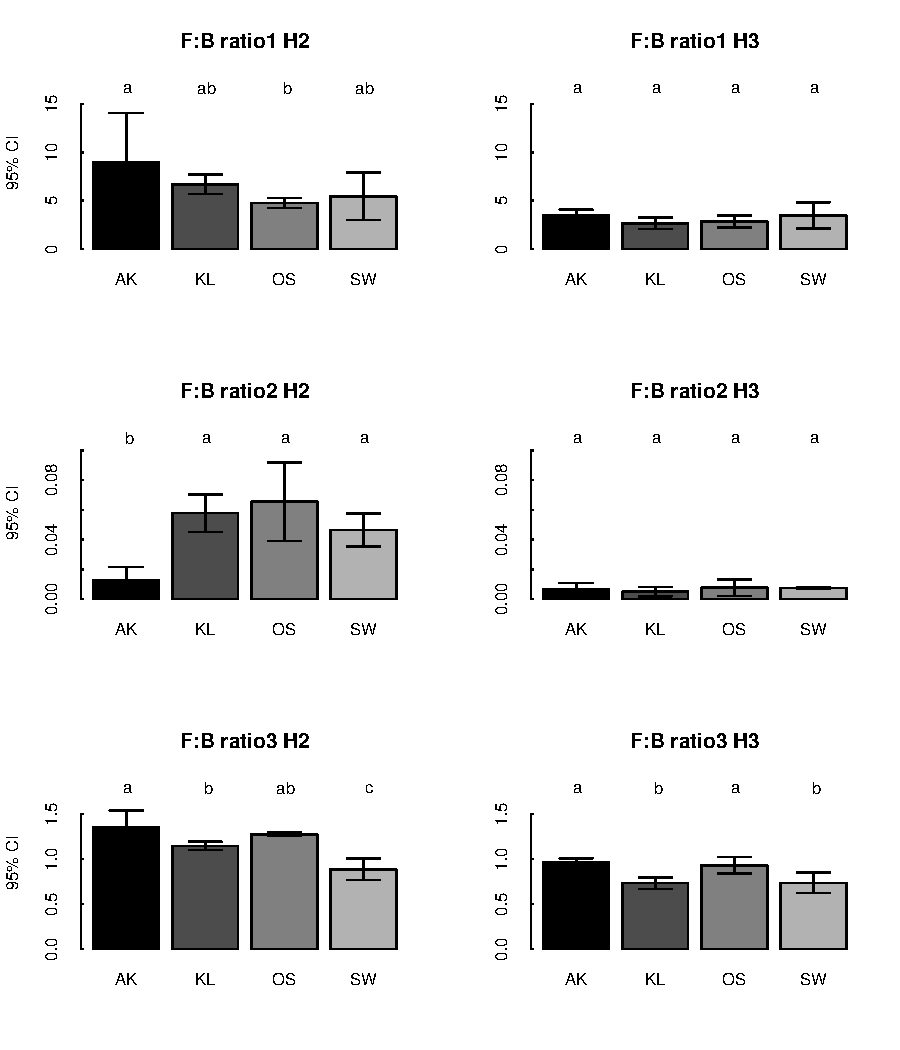
\includegraphics[width=12cm]{plfa.pdf}
% \end{center}
% \caption{Fungi : Bacteria ratios}
% \label{fig:plfa}
% \end{figure*}
